% Root document — scholarly review of acoustic significance in rodents.
% Build from the repository root via `make pdf` / `make docx` (see README.md).

\documentclass[12pt,letterpaper]{article}

% Shared packages and macros. Loaded by main.tex only.
% Do not compile this file directly.

\usepackage[utf8]{inputenc}
\usepackage[T1]{fontenc}
\usepackage{lmodern}
\usepackage[margin=1in]{geometry}
\usepackage{setspace}
\usepackage{microtype}
\usepackage{graphicx}
\usepackage{booktabs}
\usepackage{tabularx}
\usepackage{longtable}
\usepackage{pdflscape}
\usepackage{float}
\usepackage{array}
\usepackage{enumitem}
\usepackage{amsmath}
\usepackage{amssymb}
\usepackage{xcolor}
\usepackage{colortbl}
\usepackage[hidelinks]{hyperref}
\usepackage{natbib}

\graphicspath{{figures/}}

% Line spacing suitable for drafting and review
\onehalfspacing

% Convenience macros
\newcommand{\figref}[1]{Figure~\ref{#1}}
\newcommand{\tabref}[1]{Table~\ref{#1}}
\newcommand{\secref}[1]{Section~\ref{#1}}
% Supplementary-table reference; second argument is the S-number, used only by the DOCX export.
\providecommand{\stabref}[2]{Table~\ref{#1}}
% True only in the pandoc DOCX export (scripts/pandoc_flags.tex). Use at top level only.
\providecommand{\ifpandoc}{\iffalse}

% Static figure placeholder (no generated artwork). Use inside figure env before \caption.
\newcommand{\figplaceholder}[1]{%
  \centering
  \fbox{%
    \begin{minipage}[c][0.28\textheight][c]{0.92\textwidth}
      \centering
      \large\textit{Figure artwork pending}\\[0.6em]
      \normalsize #1
    \end{minipage}%
  }%
}


% Metadata for the DOCX export; the PDF uses the explicit title block below.
\title{Interpreting Acoustic Risk: Integrating Field Ethology and Laboratory Neuroscience in Rodents}
\author{Matt Gaidica \and Department of Neuroscience, Washington University School of Medicine, St.~Louis, MO 63110, USA \and gaidica@wustl.edu (corresponding author)}
\date{}

\begin{document}

\ifpandoc\else
\begin{center}
  {\LARGE Interpreting Acoustic Risk:}\\[0.35em]
  {\large Integrating Field Ethology and Laboratory Neuroscience in Rodents}\\[1.1em]
  {\large Matt Gaidica}\\[0.45em]
  {\small
    Department of Neuroscience, Washington University School of Medicine,\\
    St.\ Louis, MO 63110, USA\\
    gaidica@wustl.edu\\[0.25em]
    \textit{Corresponding author}}
\end{center}
\vspace{1em}
\fi

% Working abstract. Journal limit: 150--250 words, no undefined abbreviations or references.
\begin{abstract}
\noindent Rodents live in acoustic environments where few sounds signal danger, yet failing to respond to the right ones can be fatal. How receivers assign meaning to sound, and why that meaning persists or fades with repetition, therefore bears directly on the function and evolution of antipredator behavior. We review how ground squirrels, marmots, and other field-studied rodents, together with laboratory mice and rats, recognize, interpret, and adapt to biologically meaningful sounds, including conspecific alarm and distress calls, heterospecific alarm calls, and predator vocalizations, relative to acoustically matched artificial controls. We organize the evidence around seven questions spanning recognition, assessment and behavioral response, and updating over time. Signal detection theory, threat-sensitive predator avoidance, the economics of escape, and the predation risk allocation hypothesis frame each question by asking when responding should be favored and when responsiveness should decline. We distinguish acoustic salience from ecological significance, reflexive startle from sustained defensive behavior, and sensory habituation from learning that a signal is unreliable, and we treat neural measures such as striatal dopamine release as evidence about proximate assessment rather than direct readouts of perceived threat. We close with a receiver-centered framework linking stimulus, prior experience, assessment, response, and updating, and propose testable hypotheses, pairing field and laboratory systems, about how signal reliability and temporal predictability govern the persistence of responses to repeated sounds.
\end{abstract}

\noindent\textbf{Keywords:} alarm calls; antipredator behavior; habituation; signal reliability; risk allocation; rodents


\tableofcontents
\newpage

\section{Introduction: the challenge of acoustic significance}
\label{sec:introduction}

An animal that hears a sudden sound has to decide, often within a second, whether to act. A false alarm costs time and food; a missed threat can cost its life. These lopsided costs favor responding to anything that might signal danger \citep{Nesse2005}. They do not tell us which sounds rodents treat as significant, or whether a given sound will produce vigilance, freezing, flight, approach, a change in heart rate with no visible behavior, or nothing measurable at all.

Three observations show how puzzling this can be. Laboratory rats freeze to the 22-kHz alarm calls of other rats, but only if they have previously experienced something aversive \citep{KimEtAl2010}. They approach the 50-kHz calls that rats emit in positive social contexts, yet that approach declines rapidly with repeated playback \citep{WilluhnEtAl2014}. And juvenile Richardson's ground squirrels (\textit{Urocitellus richardsonii}) respond less to callers whose alarms are repeatedly not followed by a predator \citep{HareAtkins2001}. Acoustic meaning, in other words, is not a fixed property of a waveform, and it is not the same thing as a startle or a burst of neural activity.

This review asks how rodents recognize biologically significant sounds, how they turn acoustic information into physiological and behavioral responses, and how they revise those responses with experience and repetition. We treat laboratory mice and rats and field-studied sciurids (ground squirrels, marmots, prairie dogs, chipmunks, and gray squirrels) as complementary systems. Field work reveals natural signal use, caller identity and reliability, and ecological costs. Laboratory work offers stimulus control, developmental manipulation, and access to mechanism. The systems are not interchangeable---repertoires, hearing ranges, ecological exposure, and behavioral options differ---but they raise shared questions. Recent reviews of rodent vocalization have concentrated on production and call structure \citep{SolajaGustison2026}. Here we take the receiver's perspective, and we set field evidence on call information, caller reliability, and ecological costs directly alongside laboratory evidence on auditory, defensive, and autonomic circuits, so that each can constrain how the other is interpreted.

\subsection{Detection, interpretation, action, and updating}
\label{sec:intro-distinctions}

We distinguish four interacting processes. They are not stages of a rigid linear circuit:

\begin{enumerate}[leftmargin=*,itemsep=2pt]
  \item \textbf{Detection} --- the sound is registered as an acoustic event (e.g., startle, orienting, primary auditory responses).
  \item \textbf{Interpretation} --- the sound is assigned biological significance through predisposition, learning, or ecological familiarity.
  \item \textbf{Action selection} --- a particular overt response is expressed (freezing, flight, approach, vigilance), contingent on state and opportunity.
  \item \textbf{Updating} --- responses change with repetition, rest, caller change, reliability history, or temporal expectation.
\end{enumerate}

The list is not a fixed sequence. Some sounds bypass interpretation altogether: an abrupt or looming sound can trigger startle, freezing, or flight through short pathways that do not depend on learned meaning (\secref{sec:mechanisms-midbrain}). Detection can thus lead to action directly, in parallel with any slower evaluation of what the sound predicts.

These processes can also come apart. Amygdala neurons in naïve rats distinguish 22-kHz from 50-kHz calls, largely by frequency, while the rats do not freeze \citep{ParsanaEtAl2012a}. Spiny mice raise stress hormones to owl calls without any detectable change in behavior \citep{EilamEtAl1999}. A study that scores only freezing would classify both as ``no response.'' Such dissociations are expected if hearing, learned valuation, defensive movement, and autonomic regulation use overlapping but partly separate brain systems (\secref{sec:mechanisms}). They are central facts for any account of acoustic meaning, and laboratory freezing does not guarantee ecological consequences such as reduced foraging. \figref{fig:framework} summarizes these processes as a receiver-centered model with feedback and a parallel route from detection to action.

\begin{figure}[tbp]
  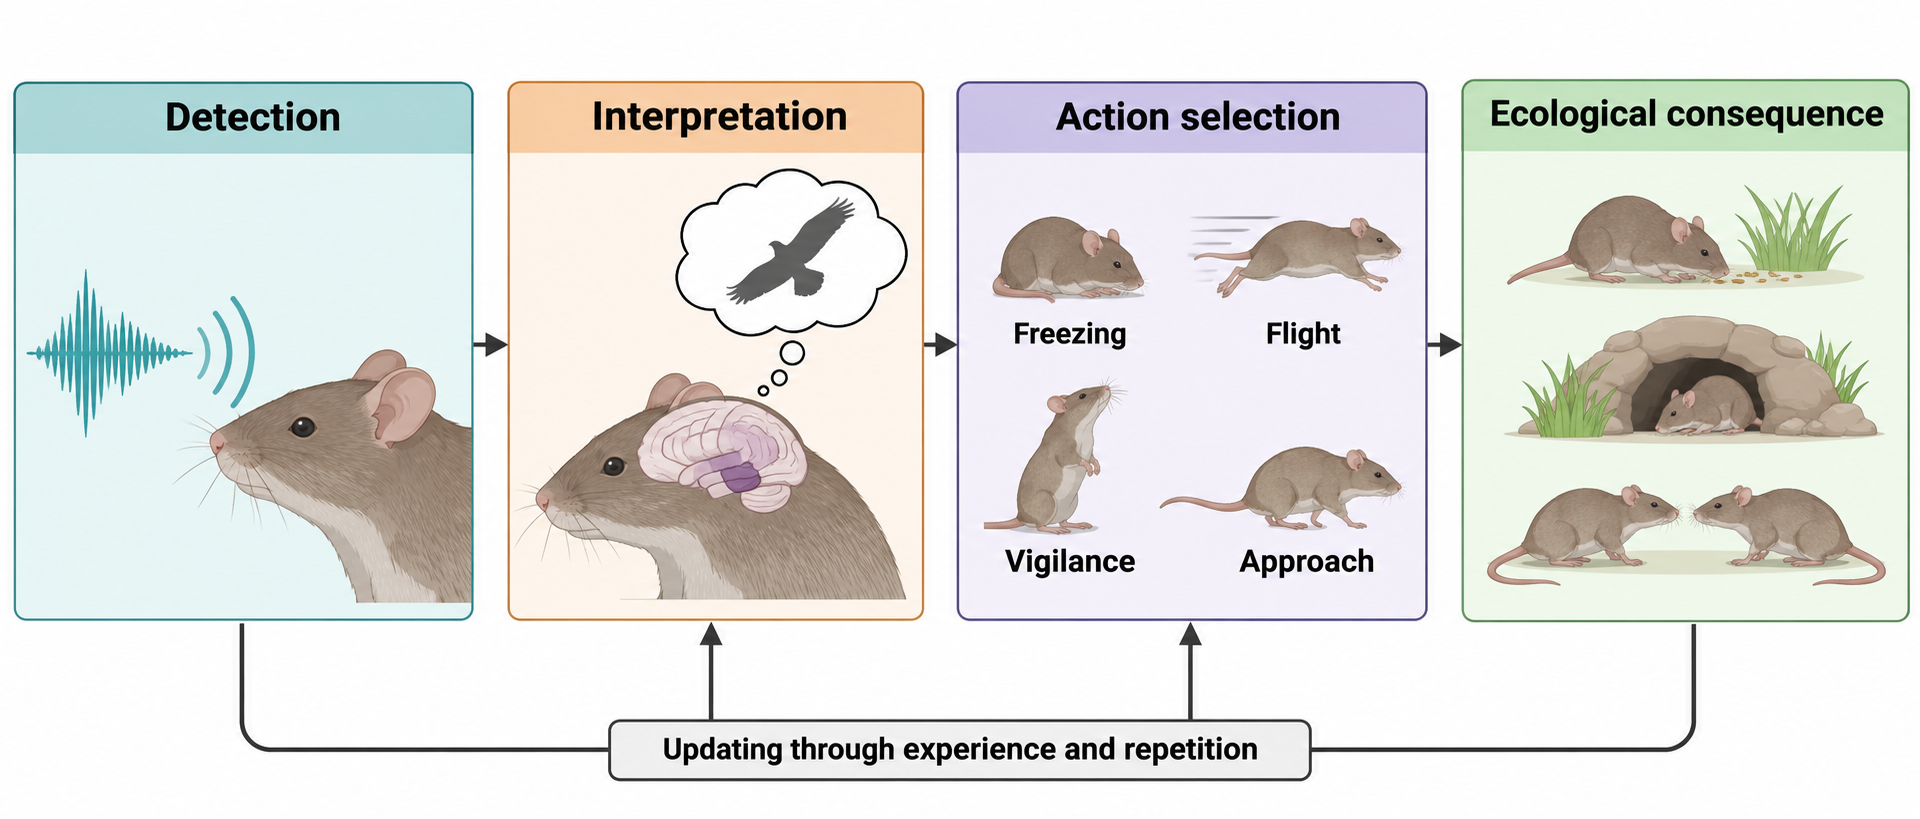
\includegraphics[width=\textwidth]{fig1_framework_placeholder.png}
  \caption{Receiver-centered conceptual model of acoustic significance (schematic). Acoustic information is interpreted in light of experience and source reliability; action depends on ecological state and decision costs; outcomes and repetition update subsequent interpretation. A parallel route links detection directly to action selection, because abrupt or looming sounds can trigger startle, freezing, or flight without learned interpretation (\secref{sec:mechanisms-midbrain}). This is not a strictly serial pathway.}
  \label{fig:framework}
\end{figure}

\subsection{Theory that frames when to respond---but not which sound}
\label{sec:intro-theory}

Functional theory explains \emph{when} receivers should respond. Threat-sensitive avoidance and the economics of escape predict that the strength and type of response should scale with assessed risk and with the relative costs of fleeing and staying \citep{Helfman1989,YdenbergDill1986}. Gray squirrels farther from refuge flee earlier from an approaching visual threat \citep{DillHoutman1989}, a spatial logic that acoustic studies rarely measure. The predation risk allocation hypothesis predicts that vigilance per high-risk period should fall when such periods are frequent \citep{LimaBednekoff1999}; it has not been tested with acoustic cues in rodents (\secref{sec:persistence}). These frameworks motivate the questions developed below. They do not identify which acoustic structures carry significance.

\subsection{Scope and contribution}
\label{sec:intro-scope}

The review concerns \textbf{rodents as receivers}: of conspecific alarm, distress, and social calls; of heterospecific alarms and safety cues; of predator vocalizations played to prey; and, as a contrast, of rat 50-kHz calls, which attract rather than alarm and so constrain any claim that meaningful natural sounds are uniformly threatening. How predators respond to rodent calls lies outside this scope. Visual and multisensory paradigms appear only where needed to delimit an acoustic finding. We do not survey vocal production or applications.

Throughout, we distinguish \textbf{empirical results}, \textbf{theoretical interpretation}, and \textbf{open hypotheses}. The contribution is a synthesis across systems of how acoustic structure, receiver history, ecological context, and updating jointly determine response, organized around three recurring demands on the receiver. It is not a demonstrated unified mechanism, and not a guide to choosing playback stimuli.

\secref{sec:features} asks what information rodents extract from sound. \secref{sec:mechanisms} follows that information into the neural and physiological systems that support, and sometimes dissociate, discrimination, valuation, defense, and changes in body state. \secref{sec:action} compares how ecological and laboratory receivers select actions, and what defensive circuits suggest about field behavior. \secref{sec:persistence} treats updating with experience and repetition. \secref{sec:account} develops an integrated account built on three recurring demands: responding rapidly to salient sounds, learning what sounds predict, and selecting actions according to context and cost. \secref{sec:outlook} identifies outstanding questions. Representative findings are summarized in \tabref{tab:comparison}, with detailed comparisons in \stabref{tab:comparison-supp}{1} and a study-level matrix in \stabref{tab:evidence-supp}{2}.

\section{What information do rodents extract from sound?}
\label{sec:features}

To say that a sound is biologically significant is to say something about a receiver: what it extracts from the sound, and how that information shapes what it does next. It is not a statement about whether the sound is ``natural'' or ``alarming.'' Studies of rodent receivers keep returning to the same acoustic dimensions: carrier frequency and bandwidth, sound level, frequency and amplitude modulation, the temporal envelope, syllable and bout structure, call rate, harsh or noisy (nonlinear) components, and cues to the caller's identity. A natural call bundles all of these. Comparing a natural call with an artificial one therefore rarely shows which property mattered. And when a simplified sound reproduces a response, it remains open whether simplification stripped away meaning or simply isolated the features that were sufficient for that response.

\subsection{Acoustic salience is not ecological meaning}
\label{sec:features-salience}

Natural calls often beat poorly matched controls but fail to beat controls matched on the features the receiver actually uses. In food-restricted rats, natural 50-kHz calls evoked approach and a transient rise in nucleus accumbens dopamine, whereas natural 22-kHz calls and noise matched in duration and amplitude evoked neither \citep{WilluhnEtAl2014}. That shows the rats distinguished calls from that noise; it does not show which acoustic property was necessary. Pure-tone approximations of 50-kHz calls, lacking natural frequency and amplitude modulation, still draw rats toward the speaker, especially adults \citep{WohrSchwarting2007}. Natural 22-kHz and 50-kHz calls generally produce larger vocal, cardiac, and locomotor effects than computer-generated tones, but in the same direction, and housing condition changes the size of the effect \citep{OlszynskiEtAl2020}. In the amygdala, frequency-matched tones reproduce most of the neural discrimination between the two call types in naïve rats \citep{ParsanaEtAl2012a}. The inference these results support is narrower than ``natural calls are special'': frequency band and gross timing often suffice for the measured response. A response to simplified tones shows that those features are sufficient for that endpoint, not that natural calls carry no further meaning, and a difference between a call and noise is not a test of which features matter.

Significance can also interact with loudness. Rats oriented more to a recorded distress squeal than to a synthetic mimic with matched timing at 100~dB, but not at 80~dB \citep{EvansHammond1983a}. A comparison at a single sound level can create or erase an apparent advantage for the natural call. Conversely, a sound can be aversive without being ecologically meaningful: a standardized synthetic 17--20~kHz sweep that resembles no natural call elicits flight or freezing in mice, depending on cage familiarity and prior shock \citep{MongeauEtAl2003}. Where studies omit calibration or hearing data, the level at the animal's ear remains uncertain.

Synthetic sounds can also acquire significance through experience. Mouse pup calls cluster around an interval of about 175~ms between syllables. Maternal experience broadens and shifts both retrieval behavior and auditory cortical tuning to synthetic calls that vary this interval \citep{SchiavoEtAl2020}. The result is specific to pup-call recognition and should not be taken as a template for other call classes. It shows that constructed sounds can become biologically effective when the manipulated feature is one a recognition system uses.

\subsection{Different alarm systems carry different kinds of information}
\label{sec:features-systems}

Field sciurids make clear that ``alarm call'' is not one informational category (\figref{fig:info-kinds}).

\begin{figure}[tbp]
  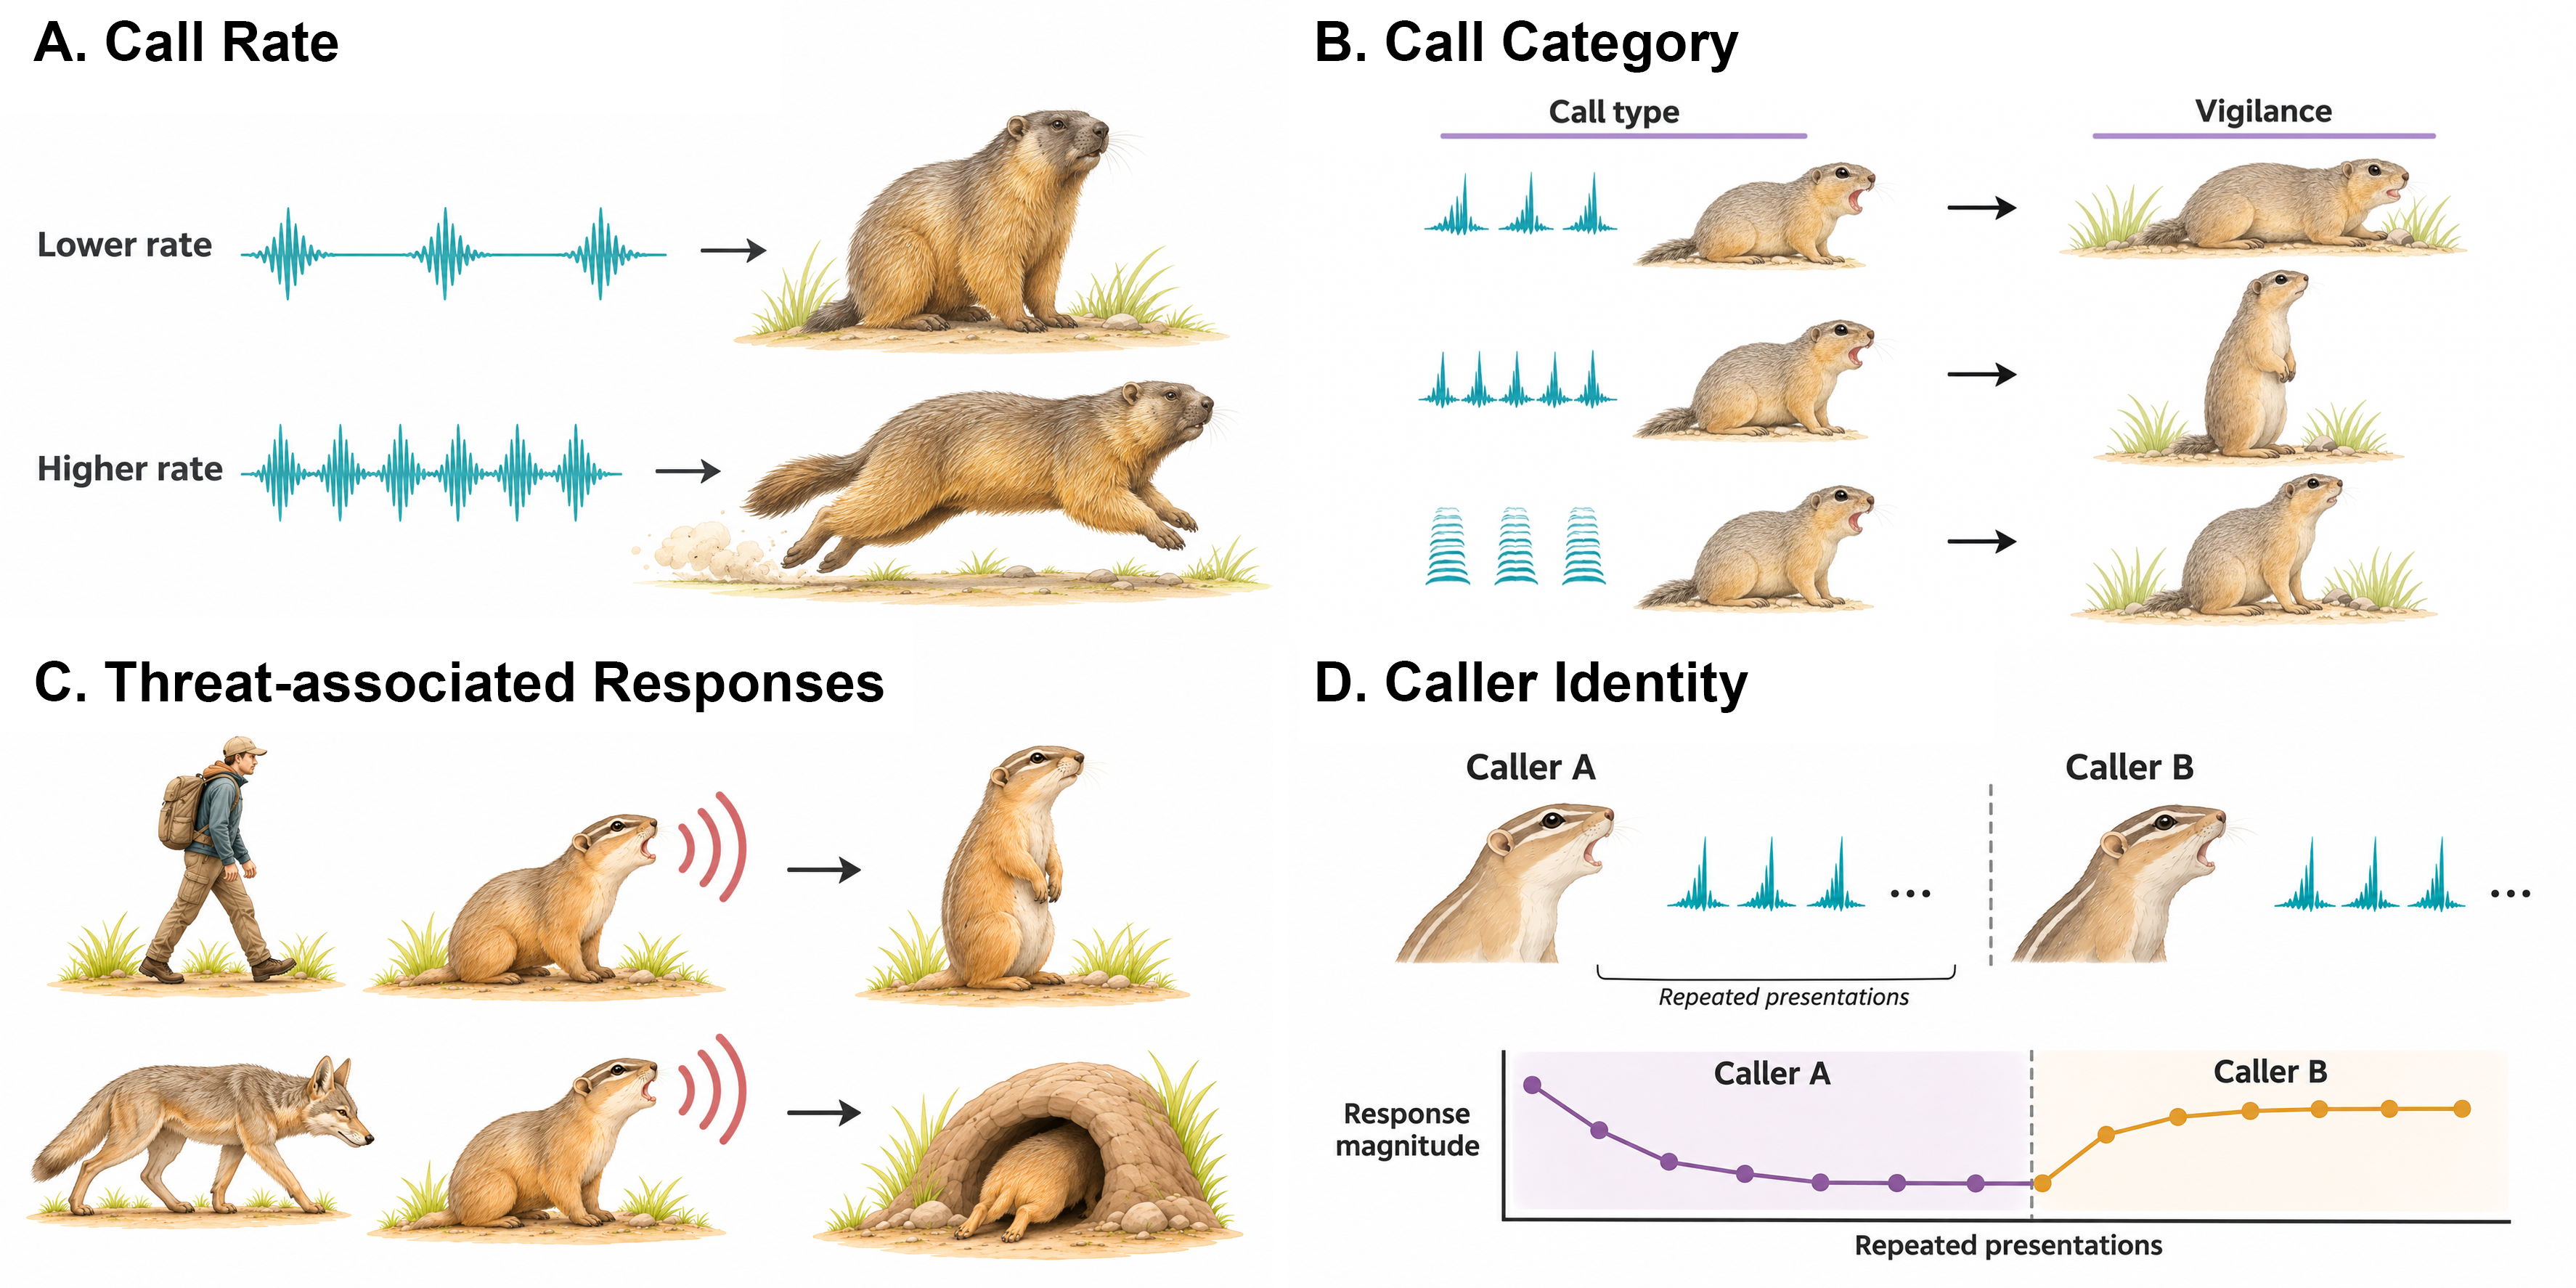
\includegraphics[width=\textwidth]{fig2_designspace.png}
  \caption{Different forms of acoustic information across rodent alarm systems. (A)~Alarm-call rate in yellow-bellied marmots conveys risk-related information, with higher rates associated with stronger antipredator responses \citep{BlumsteinArmitage1997}. (B)~Richardson's ground squirrels distinguish alarm-call categories and exhibit corresponding differences in vigilance \citep{SloanEtAl2005}. (C)~Gunnison's prairie dog alarm calls elicited by different threats, including humans and coyotes, can evoke threat-associated escape responses during playback, indicating that calls convey information beyond generalized urgency \citep{KiriazisSlobodchikoff2006}. (D)~Responses can decline across repeated presentations from one caller and recover when the caller changes, demonstrating source-specific response updating without necessarily establishing reliability learning \citep{Hare1998}. Acoustic representations, behavioral illustrations, and response curves are schematic rather than measured data; specific illustrated postures do not imply experimentally established stimulus--response mappings. Together, these examples illustrate that rodent alarm systems convey different kinds of information rather than a universal predator or urgency code. Schematic illustration created with ChatGPT (OpenAI) image generation and verified by the author.}
  \label{fig:info-kinds}
\end{figure}

Yellow-bellied marmot (\textit{Marmota flaviventer}) alarms do not map onto predator species. Instead, call rate and some acoustic parameters track risk, and receivers use rate as risk information \citep{BlumsteinArmitage1997}.
% VERIFY: BlumsteinRecapet2009, SloanEtAl2005, SwanHare2008 (not full-text checked where marked).
Adding noisy, nonlinear components to marmot calls reduces foraging more than unmanipulated calls do \citep{BlumsteinRecapet2009}. Richardson's ground squirrels adjust vigilance differently to chirps, whistles, and chucks \citep{SloanEtAl2005}, and the first syllables of repeated calls are strongly alerting \citep{SwanHare2008}. Gunnison's prairie dogs (\textit{Cynomys gunnisoni}) are a contrasting case. Playback of alarm calls previously elicited by humans, dogs, or coyotes reproduces the corresponding escape behavior, whereas a control matched in rhythm, frequency range, and amplitude does not \citep{KiriazisSlobodchikoff2006}. The calls carry enough information for predator-specific escape; this does not require that they function as words, and it has not been shown for other sciurids. Urgency coding and predator-associated categories are different informational solutions, and resisting a universal claim about ``what alarm calls mean'' is part of the comparative point.

Who is calling is itself information. Marmots respond more to juvenile than to adult-female calls but do not distinguish familiar from unfamiliar callers \citep{BlumsteinDaniel2004}. Caller identity is carried by rat 50-kHz calls \citep{VielleEtAl2021} and by prairie vole calls \citep{WarrenEtAl2025}.
% VERIFY: WarrenEtAl2025, SchmidtEtAl2008 (not full-text checked).
Nor is relevance ranked by whether the source is a predator. Eastern chipmunks (\textit{Tamias striatus}) change their foraging more to titmouse mobbing calls than to hawk calls \citep{SchmidtEtAl2008}: an indirect social cue can outweigh a predator's own voice.

\subsection{Interpretation depends on experience and social ecology}
\label{sec:features-experience}

A sound can be ecologically relevant without being recognized innately. Tests of predator-call recognition in predator-naïve laboratory rodents disagree. Male DBA/2 mice show defensive responses to owl calls \citep{HendrieNeill1991}, whereas C57BL/6J mice, Sprague-Dawley rats, and gerbils show no selective defense relative to non-predator calls \citep{KindermannEtAl2009}. Species, strain, sound level, and endpoint all differ; a lack of freezing does not mean a lack of acoustic processing; and the variation across paradigms rules out a simple innate-versus-learned answer. Rodents with field experience respond more consistently, though in different ways: voles may freeze or flee, while spiny mice show hormonal change without overt behavior \citep{EilamEtAl1999,HendrieEtAl1998}.

Rat 22-kHz calls show the role of experience most clearly. Selective freezing to these calls depends on prior aversive experience \citep{KimEtAl2010,EndresEtAl2007}, and preventing a rat from calling during its own shock does not abolish later freezing to the calls \citep{CalubEtAl2018}. Yet naïve rats still slow their movement and heart rate to natural 22-kHz calls \citep{OlszynskiEtAl2020}, so ``no response without experience'' is true only if freezing is the sole measure. In the field, eavesdropping on other species' alarms reflects both familiarity and acoustic similarity \citep{GetschowEtAl2013,Shriner1998}, and receivers also use other species' sounds as signals of safety \citep{LillyEtAl2019}.

\subsection{The generality problem}
\label{sec:features-generality}

Which of these findings reflect learned associations specific to a species, which reflect general acoustic biases (rough or abrupt sounds as attention-grabbing, for example), and which depend on social ecology? Telling these apart requires acoustically controlled variants presented to receivers with different associative histories, with the same endpoints measured in laboratory and field animals. Few studies provide both. Unmatched controls, single sound levels, unreported calibration, and strain differences are therefore not technical footnotes; they limit what can be inferred about the information a sound carries.

The same acoustic feature can also feed different downstream systems. Frequency or timing codes that support discrimination need not engage the circuits that select freezing, flight, or autonomic change, and abrupt or looming sounds can trigger defense through fast routes that bypass learned meaning (\secref{sec:mechanisms}). These tensions recur when laboratory and field receivers are compared in \secref{sec:action} and \tabref{tab:comparison}.

\section{From acoustic information to neural and physiological responses}
\label{sec:mechanisms}

A rat that hears a 22-kHz alarm call may slow its heart, stop moving, freeze, or do nothing visible at all. If acoustic significance were a single internal ``fear'' variable, these responses would rise and fall together. They often do not. The reason is anatomical as much as psychological: hearing a sound, learning what it predicts, changing body state, and choosing a defensive action recruit overlapping but partly separate brain systems. Startle, vigilance, freezing, flight, and approach are therefore not interchangeable readouts of one state, and a null on one measure is not proof that a sound went unprocessed.

This section follows acoustic information from the ear into the networks that assign significance, select actions, and adjust the body, and then asks how much of that map has been shown for natural sounds. Ecological moderators of action---refuge, foraging opportunity, social setting---are treated in \secref{sec:action}; here the focus is on the neural organization that makes dissociations expected rather than anomalous.

One distinction runs through everything that follows. Circuit neuroscience has mapped defensive pathways in remarkable detail, but mostly with \emph{synthetic or conditioned sounds}: tones, noise, or looming sounds, often given meaning by pairing with foot shock. Far fewer studies use \emph{natural vocalizations} (conspecific, heterospecific, or predator calls), and fewer still use \emph{other natural sounds} that are not vocalizations. We also separate what experiments can show: \emph{causal} studies that lesion, silence, or drive a pathway; \emph{activity} studies that record neurons or map c-Fos or fMRI signals, which are correlational; and studies of \emph{physiology or behavior} alone. A result in one stimulus class is not a demonstration in another (\figref{fig:ladder}).

\begin{figure}[tbp]
  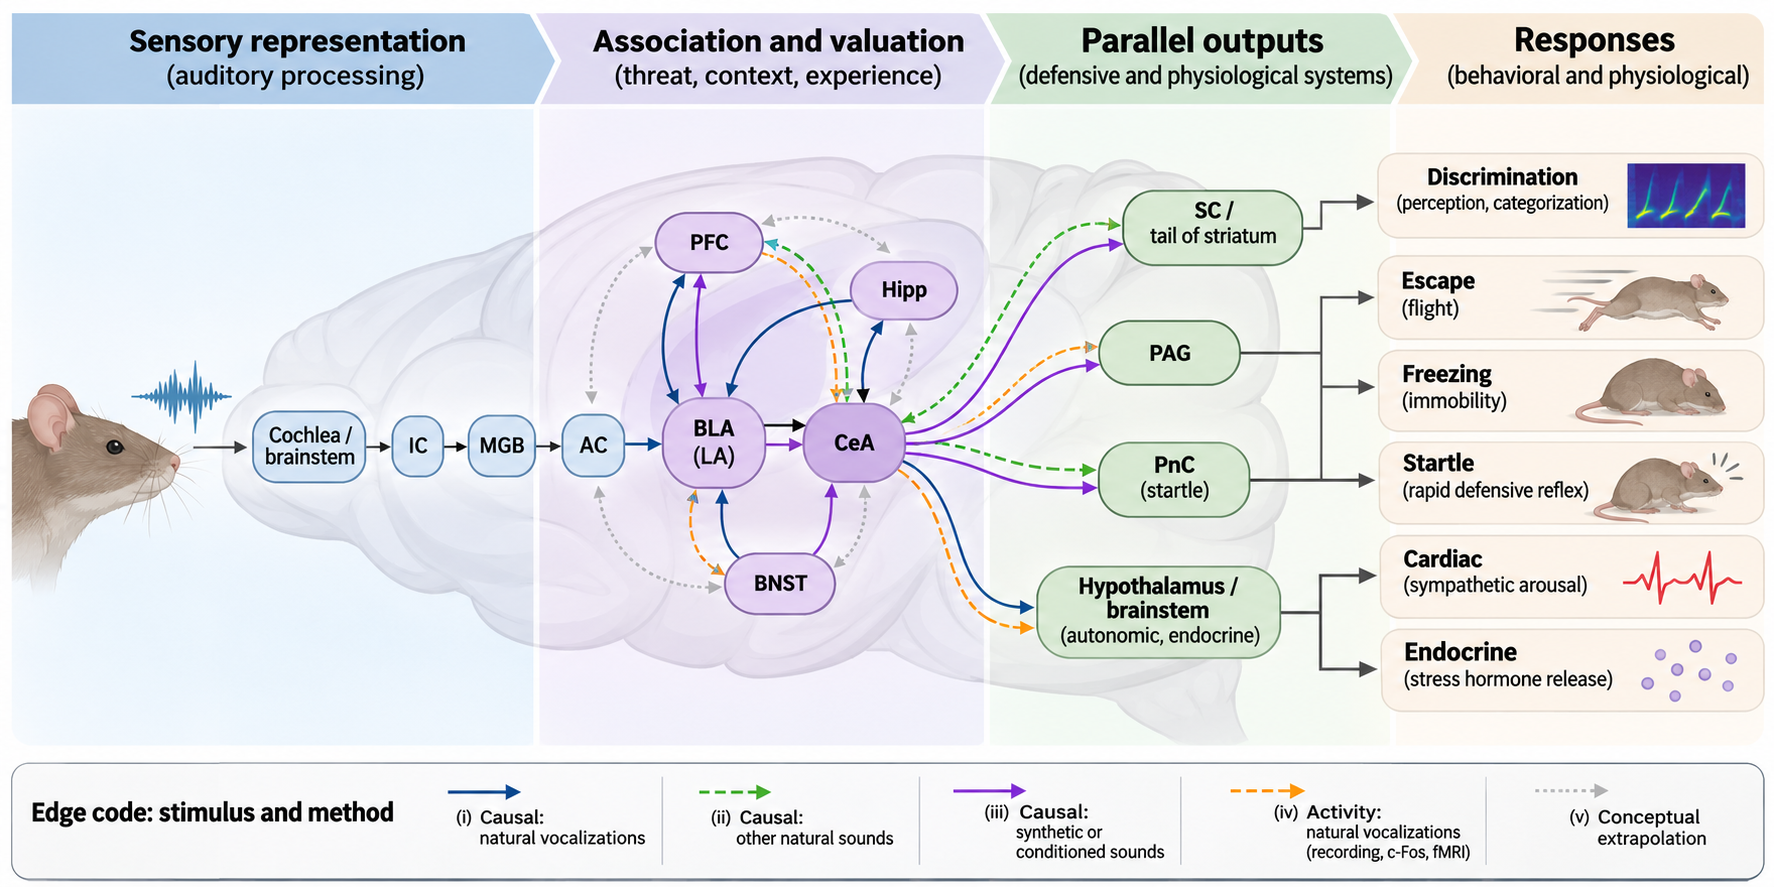
\includegraphics[width=\textwidth]{fig3_ladder_placeholder.png}
  \caption{Parallel pathways from acoustic information to physiological and defensive responses (schematic). Zones: sensory representation (cochlea/brainstem, inferior colliculus, medial geniculate body, auditory cortex); association and valuation (lateral/basolateral and central amygdala, bed nucleus of the stria terminalis, with prefrontal and hippocampal modulation); parallel outputs (periaqueductal gray, acoustic-startle route via caudal pontine reticular nucleus, superior colliculus and tail of striatum, hypothalamic and brainstem autonomic targets); and responses (discrimination, startle, freezing, escape, cardiac and endocrine change). Edges are coded by stimulus and method: (i)~causal evidence with natural vocalizations; (ii)~causal evidence with other natural sounds; (iii)~causal evidence with synthetic or conditioned sounds; (iv)~activity evidence (recording, c-Fos, fMRI) with natural vocalizations; (v)~conceptual extrapolation. Pathways are compiled across preparations; the full network has not been established as a natural alarm-call circuit in any one rodent species.}
  \label{fig:ladder}
\end{figure}

\subsection{Auditory pathways and access to defensive systems}
\label{sec:mechanisms-auditory}

How does a sound reach the parts of the brain that can make an animal afraid? The hearing pathway runs from the cochlea through brainstem nuclei to the inferior colliculus (IC) in the midbrain, then to the auditory thalamus (medial geniculate body, MGB) and auditory cortex. From thalamus and cortex, signals reach the lateral and basolateral amygdala (LA/BLA), the regions most studied when animals learn that a sound predicts danger. Along the way, neurons represent frequency, loudness, and timing. That is feature coding, not meaning. A neuron tuned to 22~kHz can tell call types apart without telling the animal whether the call currently predicts danger.

Classic lesion work in rats established that the thalamus, not the cortex, was needed for a tone paired with shock to raise blood pressure and evoke freezing: auditory cortex lesions left these conditioned responses intact, whereas MGB or IC lesions abolished them \citep{LeDouxEtAl1984}. Recordings later showed that conditioning sharpens short-latency LA responses to the tone \citep{QuirkEtAl1995}. Both studies used conditioned tones. They show that acoustic information can reach the amygdala quickly and that learning reshapes it there. They do not show that cortex is dispensable for sounds with richer structure.

A natural danger cue that is not a call makes the point. A freezing rat falls silent, and the sudden end of its movement sounds can alarm a nearby rat. Freezing to that silence requires the dorsal MGB, a ventral area of auditory cortex, and LA \citep{PereiraEtAl2020}---an ``auditory offset'' pathway that detects the end of a sound rather than its onset. This is causal evidence with another natural sound, not with a vocalization. It shows that a naturalistic cue can depend on both thalamic and cortical stages, unlike the tone in the classic experiments, and it cautions against assuming one obligatory route for every acoustic danger cue.

For natural vocalizations themselves, the evidence at this stage is mostly activity. Amygdala neurons in naïve rats respond differently to 22-kHz and 50-kHz ultrasonic vocalizations (USVs), yet tones matched in frequency reproduce most of that difference, and the rats do not freeze \citep{ParsanaEtAl2012a}. c-Fos mapping after USV playback likewise shows call-type differences in auditory and limbic regions \citep{SadanandaEtAl2008,OudaEtAl2016}, without identifying which regions are required. Sensitivity to frequency or timing is not the same as knowing what a call means.

\subsection{Amygdala circuitry for learned significance and response selection}
\label{sec:mechanisms-amygdala}

Learning that a sound predicts danger and choosing what to do about it are different problems. The amygdala contributes to both, through different components.

The first problem---association---is linked to LA/BLA. In auditory fear conditioning, the tone and the shock converge there, and synaptic inputs from thalamus and cortex are strengthened. Conditioning enhances LA responses to the tone \citep{QuirkEtAl1995} and occludes further potentiation at cortical inputs, as if the synapses had already been strengthened by learning \citep{TsvetkovEtAl2002}. These are causal and cellular findings with conditioned tones. They show how an acoustic association can be stored; they do not tell us how a natural call acquires meaning.

The second problem---selection---is linked to the central amygdala (CeA), which lies closer to output. In mice trained so that a cue shifts from a tone to a burst of white noise, two populations of CeA inhibitory neurons compete: somatostatin-expressing cells promote freezing, corticotropin-releasing-factor-expressing cells promote flight, and each suppresses the other \citep{FadokEtAl2017}. The circuit offers a mechanism for switching rapidly between passive and active defense. It was demonstrated with conditioned sounds, so it is a candidate mechanism for natural calls, not a demonstrated alarm-call pathway. It also shows that even CeA is not a single ``fear center''; competing outputs sit within it.

Rat 22-kHz calls show what experience adds. Rats freeze selectively to a distressed partner's 22-kHz calls only if they have previously experienced shock, and this social transmission of fear requires the auditory thalamus \citep{KimEtAl2010}. The design used a live sender, so multiple cues were available; the causal claim is about thalamic integrity and prior experience, not a complete pathway from LA through CeA. Preventing the receiver from calling during its own shock does not abolish later freezing \citep{CalubEtAl2018}, so hearing oneself call is not required. Meanwhile, naïve rats still slow their heart and locomotion to the same calls \citep{OlszynskiEtAl2020}. Discrimination and bodily response can thus exist without freezing; experience gates the action, not necessarily the perception.

\subsection{Midbrain and brainstem: startle, freezing, and escape}
\label{sec:mechanisms-midbrain}

A sudden noise can make a rodent flinch, freeze, or bolt. These look like points on one scale of alarm, but they arise from at least three distinct families of circuits.

The fastest is the acoustic startle reflex. A short pathway from cochlear root neurons to the caudal pontine reticular nucleus (PnC) in the brainstem, and from there to spinal motor neurons, produces the whole-body flinch within milliseconds \citep{DavisEtAl1982,LeeEtAl1996}. State and learning can modulate startle amplitude, and fear-potentiated startle uses this as a probe of conditioned fear. But a startle shows that a sound was loud and abrupt, not that it was recognized as dangerous.

The second family produces freezing. The periaqueductal gray (PAG) is a midbrain region that organizes defensive movements. In mice, inhibitory projections from CeA to ventrolateral PAG release PAG output neurons, which drive premotor targets in the medulla to produce freezing; this freezing pathway interacts with circuits for flight \citep{TovoteEtAl2016}. The pathway was defined with conditioned sounds and optogenetic manipulation. It explains how a learned acoustic cue can stop an animal in its tracks. It has not been tested for natural calls, or for sciurid vigilance or prairie-dog escape.

The third family drives active escape, and it need not pass through the amygdala at all. Neurons in auditory cortex that project to the IC can trigger flight when activated optogenetically, and silencing them reduces sound-evoked flight; their targets in the IC in turn project to dorsal PAG \citep{XiongEtAl2015}. Sounds that grow louder, mimicking an approaching object, elicit freezing followed by flight in mice: freezing depends on cortical projections to the tail of the striatum, flight on projections to the superior colliculus (SC), and the switch tracks the different time courses of the two targets \citep{LiEtAl2021}. Both studies used synthetic sounds. What they add is architectural: the auditory cortex can drive defense directly, through parallel descending routes, without first assigning learned meaning.

Predatory imminence theory offers a functional frame for these families: animals shift from vigilance to freezing to escape as a threat is judged nearer \citep{Fanselow1994}. The theory organizes defensive priorities. It is not a wiring diagram, and it has not been mapped onto circuits in wild sciurids. Which family a given sound engages depends on the sound, the animal's state, and what the experiment measured (\secref{sec:action}).

\subsection{Autonomic and endocrine channels and extended amygdala}
\label{sec:mechanisms-autonomic}

A sound can change an animal's body without changing its behavior. To see why, it helps to recall how the body's defensive physiology is controlled. The autonomic nervous system has two branches: sympathetic output raises heart rate and blood pressure and mobilizes energy, while parasympathetic output, carried largely by the vagus nerve, slows the heart. The hypothalamic--pituitary--adrenal (HPA) axis acts more slowly: the paraventricular nucleus of the hypothalamus (PVN) triggers a hormonal cascade that ends in glucocorticoid release from the adrenal glands over minutes. Limbic regions, including the amygdala, prefrontal cortex, and hippocampus, shape both systems through relays in the hypothalamus and brainstem, which lets prior experience tune the stress response \citep{UlrichLaiHerman2009}.

These controls run partly in parallel with the motor circuits for defense. In rats given tone--shock conditioning, lesions of the lateral hypothalamus disrupted the conditioned rise in blood pressure but spared freezing, whereas lesions of the midbrain central gray (the PAG) disrupted freezing but spared the blood-pressure response \citep{LeDouxEtAl1988}. Different CeA targets, in other words, carry the cardiovascular and behavioral components of the same learned response. The heart is also a misleading readout on its own. A conditioned tone and an unpaired control tone raised heart rate by the same amount, but by different means: combined sympathetic and parasympathetic drive in conditioned rats, sympathetic drive alone in controls \citep{IwataLeDoux1988}. The same heart rate can hide different physiology.

Direction matters too. Freezing is typically accompanied by a slowing of the heart, a parasympathetic brake that may support attention and preparation for action, whereas flight is accompanied by sympathetic acceleration \citep{Roelofs2017}. Natural calls fit this pattern without settling its mechanism. In rats, 22-kHz calls abruptly lowered heart rate and locomotion, whereas 50-kHz calls raised both, and natural calls had stronger effects than matched tones \citep{OlszynskiEtAl2020}. Juvenile Belding's ground squirrels discriminate alarm call types by heart rate before they discriminate them behaviorally \citep{Mateo1996,Mateo2010}.
% VERIFY: Mateo1996, Mateo2010 (not full-text checked).
Spiny mice raise cortisol to owl calls without detectable freezing or flight, whereas voles show both hormonal and behavioral change \citep{EilamEtAl1999}. These are physiology-and-behavior studies with natural vocalizations; they show what changes, not which pathway changed it.

The bed nucleus of the stria terminalis (BNST), part of the ``extended amygdala,'' is often described as the seat of sustained anxiety. Causal work shows something more specific: BNST is needed for freezing to threat cues that poorly predict when shock will arrive \citep{GoodeEtAl2019}. That suggests a role in uncertainty, which may matter for alarm calls whose reliability varies, but the link has not been tested. During USV playback, BNST- and BLA-related activity differs between 22- and 55-kHz calls in c-Fos and awake fMRI studies \citep{DemaestriEtAl2019,GranataEtAl2024}. This is activity evidence; it locates engagement without establishing necessity.

Autonomic and endocrine change can therefore diverge from behavior because different efferent systems and timescales carry them. That is why a hormone rise is not automatically ``fear,'' why a behavioral null need not mean the sound was ignored, and why a single peripheral measure cannot stand in for an ecological decision. Field physiology has nonetheless relied mainly on glucocorticoids to assess how animals respond to stressors. Heart rate and heart rate variability index sympathetic--adrenal--medullary activation more directly, can complement glucocorticoid measures, and can now be recorded in free-living animals with miniaturized biologgers \citep{GaidicaDantzer2020}. For acoustic risk, that opens a practical bridge between fields: the autonomic dissociations that laboratory studies reveal could be measured in wild receivers as they hear natural calls under realistic costs.

\subsection{Context, learning, and neuromodulatory state}
\label{sec:mechanisms-state}

The same sound does not always mean the same thing. A rat may freeze to a tone in one context and not another; a mother may ignore pup calls before giving birth and run toward them after. Two kinds of mechanism shape this flexibility: forebrain circuits that decide whether a sound matches what was learned, and neuromodulators that set the gain and readiness of the whole system.

Prefrontal cortex and hippocampus help decide how far learned fear should generalize. In rats trained to fear one tone, auditory cortex and the prelimbic region of prefrontal cortex synchronize when a new, safe tone is played, and the strength of that synchrony predicts whether the animal withholds freezing; silencing auditory cortex input to prelimbic cortex, but not to BLA, made rats generalize fear to the new tone \citep{ConcinaEtAl2018}. Dorsal hippocampal lesions had the opposite effect, sharpening discrimination after extensive training \citep{QuinnEtAl2009}. Prefrontal subregions also divide labor: inactivating prelimbic cortex reduced expression of conditioned fear, whereas inactivating infralimbic cortex impaired extinction learning, and ventral hippocampus contributed to both \citep{SierraMercadoEtAl2011}. All of this comes from conditioned tones. It is nonetheless directly relevant to the receiver's problem in the field: whether to treat a new caller or a variant call like a known alarm is a generalization decision.

Neuromodulators adjust how strongly a sound drives behavior. Norepinephrine from the locus coeruleus (LC) helps convert a retrieved auditory fear memory into freezing in conditioned mice \citep{DuanEtAl2025}.
% VERIFY: DuanEtAl2025 stimulus and causal claims against primary text.
Arousal that makes a remembered cue effective is not the same as learning that a particular caller is unreliable. Dopamine shows regional and preparation dependence rather than a threat signal: natural 50-kHz calls transiently raise nucleus accumbens dopamine along with approach, whereas 22-kHz calls do not \citep{WilluhnEtAl2014}, and dopamine responses to noise depend on region, intensity, and whether the noise was predicted, in ways that disagree across preparations \citep{GoedhoopEtAl2022,FuruyamaEtAl2026}. Dopamine is informative about valence and prediction, not a stand-in for alarm-call circuits.

Pup calls offer a revealing non-threat contrast. In mice, oxytocin acting in auditory cortex enables pup-retrieval behavior and rebalances cortical inhibition so that pup calls become more salient \citep{MarlinEtAl2015}. This is causal evidence with natural vocalizations, and it concerns care rather than defense. It shows that neuromodulation can retune how natural calls are heard, and that biologically significant sound is not synonymous with threat.

These mechanisms bridge to the experience- and repetition-dependent updating treated in \secref{sec:persistence}. Generalization, extinction, and neuromodulatory gain are candidate substrates for responses to repeated or unreliable alarms. The circuits that implement caller-reliability updating in wild sciurids remain uncharacterized.

\subsection{What has actually been demonstrated with natural acoustic signals?}
\label{sec:mechanisms-natural}

The circuit map above is impressive. How much of it has been shown for the sounds rodents actually hear in nature? Only part, and the gaps fall in predictable places.

With natural vocalizations, the evidence is strongest for behavior and physiology, weaker for neural activity, and thinnest for causation. Experience-gated freezing to 22-kHz calls, with a causal requirement for the auditory thalamus, is the clearest causal result for a defensive call \citep{KimEtAl2010}. Amygdala recordings and c-Fos maps show call-type differences, some of them stronger for natural calls than for artificial versions matched in frequency and timing \citep{ParsanaEtAl2012a,SadanandaEtAl2008,OudaEtAl2016}. Awake fMRI and c-Fos studies place extended-amygdala engagement during USV playback \citep{DemaestriEtAl2019,GranataEtAl2024}. Autonomic and behavioral measures dissociate across experience and species \citep{OlszynskiEtAl2020,Mateo1996,EilamEtAl1999}. Outside defense, oxytocin-dependent plasticity for pup calls \citep{MarlinEtAl2015} and dopamine responses to 50-kHz calls \citep{WilluhnEtAl2014} show that natural meaning need not be aversive.

With other natural sounds, the evidence is causal but narrow: the thalamic, cortical, and amygdala requirement for freezing to movement-sound cessation \citep{PereiraEtAl2020}.

Field sciurids add a further limit. In Richardson's ground squirrels, chirp and whistle playback produced call-specific c-Fos patterns, including \emph{reduced} labeling in some amygdala and collicular regions relative to no-call controls \citep{FreemanEtAl2020}. Lower c-Fos is not proof of inhibition or of a defensive pathway. The urgency coding, predator-associated categories, and caller reliability documented in marmots, prairie dogs, and ground squirrels (\secref{sec:features}; \secref{sec:action}; \secref{sec:persistence}) pose sharp neural questions that no circuit study has yet addressed.

The causal architecture---CeA competition between freezing and flight, the CeA--PAG freezing pathway, cortical and collicular escape routes, prefrontal control of generalization---comes from synthetic or conditioned sounds \citep{FadokEtAl2017,TovoteEtAl2016,XiongEtAl2015,LiEtAl2021,ConcinaEtAl2018}. None of it has been traced during naturally emitted alarms. Natural acoustic signals have well-documented, context-dependent effects on behavior; the pathways that map them onto valuation, autonomic responses, and ecological action remain far less characterized than those for laboratory threats. That gap is why a comparative field--laboratory perspective is necessary, and \secref{sec:account} uses the circuit evidence to sharpen what the field comparisons predict.

\section{From perceived risk to action: ecological and laboratory comparisons}
\label{sec:action}

A marmot that hears an alarm call can look up, stop feeding, or run for its burrow. Recognizing that a sound signals risk does not settle which of these it will do. Freezing, flight, vigilance, delayed re-emergence, and reduced foraging differ in cost and consequence, and laboratory and field settings differ in whether those costs exist at all. Comparing laboratory and field receivers shows how much the choice of action depends on those costs, and the defensive circuits of \secref{sec:mechanisms} offer hypotheses about the patterns seen in the wild (representative contrasts are in \tabref{tab:comparison}).

\subsection{Graded versus categorical responses}
\label{sec:action-graded}

Some rodents respond to alarm calls along a sliding scale; others choose among distinct actions. Yellow-bellied marmots treat call rate as information about risk, and adding harsh, noisy components to calls further suppresses foraging \citep{BlumsteinArmitage1997,BlumsteinRecapet2009}. Richardson's ground squirrels adjust vigilance differently to chirps, whistles, and chucks \citep{SloanEtAl2005}. Gunnison's prairie dogs are different: playback of alarm calls previously elicited by humans, dogs, or coyotes reproduces the matching escape patterns, whereas a control matched in rhythm, frequency, and amplitude does not \citep{KiriazisSlobodchikoff2006}. These are different informational solutions. Treating all sciurid alarms as predator labels, or all as urgency signals, misreads the comparative evidence (\secref{sec:features}).

Predatory imminence theory offers one way to relate the two patterns. It treats vigilance, freezing, and escape as distinct defensive modes that an animal enters as a threat is judged nearer, rather than as points on a single intensity scale \citep{Fanselow1994}. On that view, graded vigilance adjusts behavior within a mode, whereas categorical escape selects between modes. The framework is functional; whether sciurids implement it with the midbrain circuits studied in laboratory mice is unknown.

\subsection{Action choice depends on context and state}
\label{sec:action-context}

The same sound can produce opposite actions. Mice exposed to trains of 17--20~kHz frequency sweeps at 85~dB either flee or freeze; the two responses are negatively correlated across animals, and cage familiarity and prior foot shock shift the balance between them \citep{MongeauEtAl2003}. The sound is synthetic, which is the point: the result isolates state and opportunity from any meaning carried by the call, and the trade-off between flight and freezing is what a competition between defensive output systems would produce (\secref{sec:mechanisms-amygdala}). Experience shows a similar dissociation for natural calls. Rats freeze selectively to 22-kHz calls only after aversive experience \citep{KimEtAl2010,EndresEtAl2007}, yet they slow their movement and heart without that history \citep{OlszynskiEtAl2020}.

Field receivers weigh refuge, food, and social setting in the same way. Alarm playback makes chipmunks more vigilant, shortens their runs to cover, delays re-emergence, and reduces intake \citep{BaackSwitzer2000}; gray squirrels hearing predator calls delay and reduce foraging without changing how far they stray from refuge \citep{JayneEtAl2015}.
% VERIFY: BaackSwitzer2000, JayneEtAl2015 (not full-text checked).
In both laboratory and field, prior pairing of sound with danger shapes later action: experience gates freezing to 22-kHz calls \citep{KimEtAl2010}, and a receiver's history with particular callers revises its vigilance \citep{HareAtkins2001,BlumsteinEtAl2004}. The question is shared; the circuits need not be.

\subsection{What defensive circuits suggest about field responses}
\label{sec:action-circuits}

To our knowledge, no study has causally established the circuits that mediate natural alarm-call responses in sciurids. Playback has revealed region-specific neural activation in captive ground squirrels \citep{FreemanEtAl2020}, but recordings or manipulations of defensive circuits during alarm responses in free-ranging sciurids remain unreported. Such recordings are becoming feasible: an implantable platform that logs brain activity and movement has been demonstrated in a captive fox squirrel \citep{GaidicaDantzer2022}. The laboratory circuitry is still useful for field biology, because it shows that different behavioral outcomes can place different demands on the receiver, and those demands make predictions that field experiments can test. Three contrasts stand out. Each is a hypothesis; none has been shown to rest on the same circuits in sciurids.

\textbf{Harsh, abrupt sounds and graded vigilance.} In laboratory mice, loud or looming sounds trigger defense through fast, largely experience-independent routes---the brainstem startle pathway and cortical projections to the IC and SC---without first assigning learned meaning \citep{DavisEtAl1982,XiongEtAl2015,LiEtAl2021}. Marmots respond more strongly to calls with added noisy, nonlinear components \citep{BlumsteinRecapet2009}. If those components act through a similar arousal route, their effect should appear in inexperienced animals, generalize across callers, and decline like sensory habituation. If instead marmots have learned that harsh calls signal higher risk, the effect should depend on experience and be specific to callers whose calls have been paired with danger. Rate-based urgency information \citep{BlumsteinArmitage1997} could follow either pattern; separating harshness from rate would distinguish them.

\textbf{Predator-specific escape and action selection.} Prairie-dog escape that matches the predator type \citep{KiriazisSlobodchikoff2006} requires the receiver to evaluate a call category and select among distinct motor programs. Laboratory circuits show how such selection could work: competing CeA populations bias conditioned freezing versus flight \citep{FadokEtAl2017}, and separate cortical outputs to the striatum and the SC support freezing and flight to the same looming sound \citep{LiEtAl2021}. These results suggest a prediction for the field. If call evaluation and action selection are separable, reducing access to refuge should change the escape topography a given call elicits while leaving signs of recognition---orientation, vigilance, or cardiac change---intact.

\textbf{Vigilance, freezing, and the heart.} Vigilance (an upright scanning posture that trades feeding time for information) and freezing (immobility) are often scored as alternative ``fear'' responses. In laboratory animals, freezing comes with a parasympathetic slowing of the heart that may aid perception and preparation for action, whereas flight comes with sympathetic acceleration \citep{Roelofs2017}. Cardiac discrimination of alarm call types in juvenile ground squirrels \citep{Mateo1996} shows that heart rate can be measured in field-relevant receivers. Whether alarm-evoked vigilance carries the cardiac signature of freezing, of flight, or neither is unknown, and the answer would show whether vigilance is a form of freezing adapted for information gathering or a distinct mode.

\subsection{Heterospecific information and safety signals}
\label{sec:action-hetero}

Rodents listen to other species as well as their own. Marmots and ground squirrels respond to heterospecific alarms much as they do to conspecific alarms, relative to birdsong controls \citep{Shriner1998}; Cape ground squirrels are as vigilant to crowned-lapwing alarms as to their own species' alarms \citep{WatermanMai2020}; and gray squirrels respond more to familiar bird alarms, and to unfamiliar alarms that sound similar, than to unfamiliar dissimilar alarms \citep{GetschowEtAl2013}.
% VERIFY: Shriner1998, WatermanMai2020, LillyEtAl2019 (not full-text checked where marked).
Sounds can also signal safety. After a hawk call, ordinary bird chatter lets squirrels relax vigilance faster than ambient noise does \citep{LillyEtAl2019}. And predator source is a poor guide to impact: chipmunks change foraging more to titmouse mobbing calls than to hawk calls \citep{SchmidtEtAl2008}. Social ecology expands the set of meaningful sounds, but it also confounds familiarity with acoustic similarity unless both are manipulated.

\subsection{Costs, consequences, and where lab--field translation breaks down}
\label{sec:action-costs}

Vigilance, freezing, escape, slow recovery, and reduced foraging are not equivalent biological effects. Vigilance buys information at the cost of food; escape interrupts feeding and may expose the animal; a hormonal response without visible defense may still reflect assessment \citep{EilamEtAl1999}. A laboratory cage that offers neither food nor refuge cannot show ecological impact, however strong the freezing. Nor can ecological choices be read from neural activity in a conditioned laboratory animal, or from a single peripheral measure such as heart rate or c-Fos (\secref{sec:mechanisms}). In the other direction, field playback without matched acoustic controls or measured sound level at the receiver cannot attribute effects to particular acoustic features (\secref{sec:features}).

Temporal structure links the two settings in a similar way. Laboratory startle and amygdala responses habituate less to irregularly than to regularly timed sounds \citep{Davis1970,HerryEtAl2007}, and field responses recover when the caller changes \citep{Hare1998}. Both concern how the history of a sound shapes the next response (\secref{sec:persistence}), but laboratory timing effects with artificial sounds do not establish how natural calls should be timed to sustain field responses.

\subsection{Predator calls to prey, and the limits of attraction evidence}
\label{sec:action-scope}

Predator calls played to rodents give conflicting results in predator-naïve laboratory stock \citep{HendrieNeill1991,KindermannEtAl2009} and more consistent but still species-variable results in field-experienced animals \citep{HendrieEtAl1998,EilamEtAl1999}. Rat 50-kHz playback provides the appetitive contrast: approach and a transient rise in accumbens dopamine relative to matched noise \citep{WilluhnEtAl2014,WohrSchwarting2007}. That is attraction of laboratory rodents to conspecific calls, not evidence for field attraction in sciurids. The comparison here is how rodents respond to the sounds of predators and of conspecifics; how predators respond to the calls of their prey is a different problem.

% Main-text summary of recurring principles. Dense comparison: supplement/table_comparison_detail.tex.
\begin{table}[tbp]
\centering
\footnotesize
\singlespacing
\setlength{\tabcolsep}{5pt}
\renewcommand{\arraystretch}{1.3}
\caption{Recurring principles across laboratory and field rodent receivers. Each row states one point, the evidence that best illustrates it, and what that evidence does not establish. Fuller comparisons are in \stabref{tab:comparison-supp}{1}; study details are in \stabref{tab:evidence-supp}{2}.}
\label{tab:comparison}
\begin{tabular}{@{}>{\raggedright\arraybackslash}p{1.35in}>{\raggedright\arraybackslash}p{3.0in}>{\raggedright\arraybackslash}p{1.75in}@{}}
\toprule
\textbf{Principle} & \textbf{Illustrative evidence} & \textbf{What it does not show} \\
\midrule
Simple acoustic features often suffice
  & Tones approximating 50-kHz calls draw rats to the speaker, and frequency-matched tones reproduce most amygdala discrimination between call types \citep{WohrSchwarting2007,ParsanaEtAl2012a}.
  & That natural calls carry no further meaning. \\
Alarm calls carry different kinds of information
  & Marmot alarms grade risk by call rate; prairie-dog alarms specify escape suited to the predator \citep{BlumsteinArmitage1997,KiriazisSlobodchikoff2006}.
  & A single code shared across sciurids. \\
Experience gates action more than perception
  & Rats freeze to 22-kHz calls only after aversive experience, yet naïve rats still slow their heart and movement \citep{KimEtAl2010,OlszynskiEtAl2020}.
  & Whether predator calls are recognized without experience; tests conflict. \\
The body can respond without behavior
  & Spiny mice raise cortisol to owl calls without freezing or flight; young ground squirrels discriminate alarms by heart rate before they do so behaviorally \citep{EilamEtAl1999,Mateo1996}.
  & Which pathway produces the physiological change. \\
Parallel brain pathways allow these dissociations
  & Separate circuits support learned association, freezing, flight, and blood-pressure change \citep{LeDouxEtAl1988,FadokEtAl2017,TovoteEtAl2016,LiEtAl2021}.
  & That natural alarms use these circuits; most were mapped with tones or synthetic sounds. \\
Context selects the action
  & The same sound evokes flight or freezing depending on setting, and field receivers trade vigilance against foraging and refuge \citep{MongeauEtAl2003,BaackSwitzer2000}.
  & How costs are weighed in the brain. \\
Receivers track caller reliability
  & Ground squirrels discount unreliable callers, whereas marmots scrutinize them more closely \citep{HareAtkins2001,BlumsteinEtAl2004}.
  & Why the direction differs between species. \\
Declining responses have several causes
  & Responses recover when the caller changes, and irregular timing slows habituation to artificial sounds \citep{Hare1998,Davis1970,HerryEtAl2007}.
  & Which process underlies a given decline curve. \\
Meaningful sounds need not be threatening
  & Rats approach 50-kHz calls with a rise in accumbens dopamine, and oxytocin in auditory cortex enables mice to retrieve calling pups \citep{WilluhnEtAl2014,MarlinEtAl2015}.
  & Attraction to calls in free-living sciurids. \\
\bottomrule
\end{tabular}
\end{table}


\section{Why does the meaning or effect of a sound change with experience and repetition?}
\label{sec:persistence}

Play an alarm call to a ground squirrel and it looks up. Play the same call again and again, and it soon goes back to feeding. That decline is biologically informative, not just a practical nuisance, because the first response and the maintained response can reflect different computations. At least four accounts produce declining curves: sensory habituation; learning that a particular caller or cue is unreliable; a shift in motivation or context that makes the sound less relevant; and temporal prediction or risk allocation. Formal criteria for habituation---stimulus specificity, spontaneous recovery, dishabituation---rule out fatigue and sensory adaptation \citep{RankinEtAl2009}, but they do not separate the other three. Similar curves do not identify a single mechanism (\figref{fig:temporal}).

\begin{figure}[tbp]
  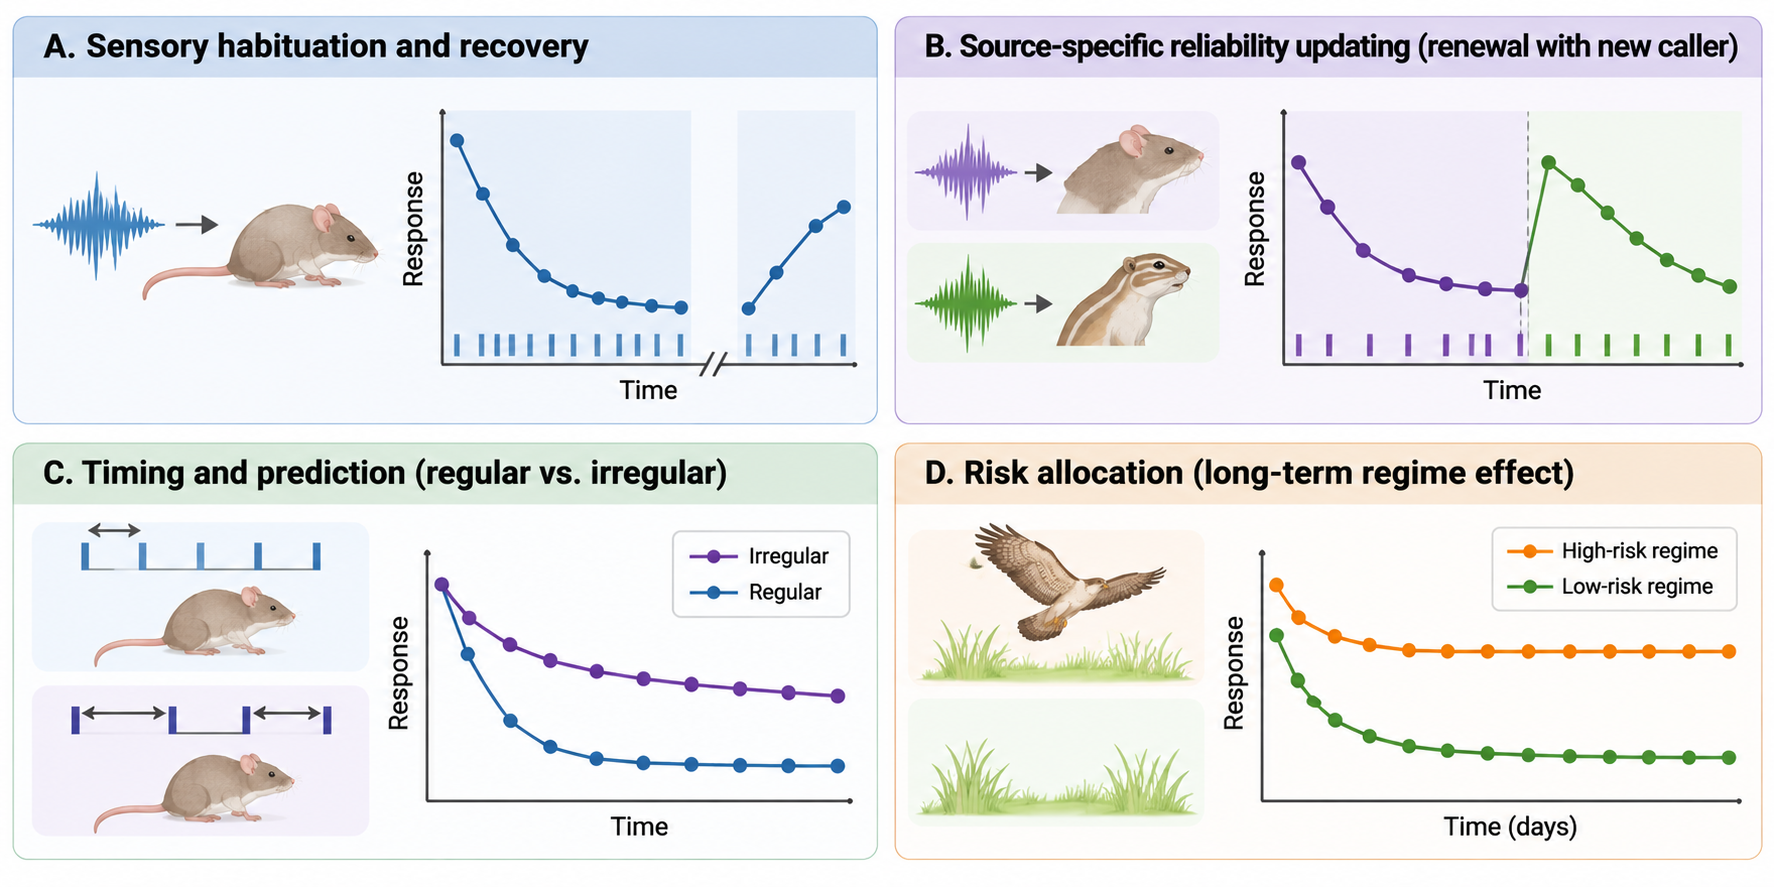
\includegraphics[width=\textwidth]{fig4_temporal_placeholder.png}
  \caption{Competing interpretations of response decline (schematic; curves idealized). (A)~Sensory habituation and recovery. (B)~Source-specific decline and renewal when the caller changes; renewal is consistent with, but does not by itself establish, reliability learning. (C)~Timing and prediction effects documented with artificial laboratory sounds. (D)~Risk allocation as a hypothesized long-term regime effect: when high-risk periods are frequent, vigilance per alarm is predicted to be lower than when they are rare. Similar curves do not identify a single process.}
  \label{fig:temporal}
\end{figure}

\subsection{Sensory habituation and recovery}
\label{sec:persistence-habituation}

Field evidence for decline specific to a caller or stimulus is strong. Richardson's ground squirrels and yellow-bellied marmots respond less across repeated calls from one individual and recover when the caller changes; in ground squirrels, a new recording from the same caller is not enough to restore responding \citep{Hare1998,BlumsteinDaniel2004}. Whether ecological significance slows habituation relative to an acoustically matched control is less clear. The main evidence is greater recovery after rest to a loud natural distress squeal than to its synthetic mimic \citep{EvansHammond1983a}. Significance does not prevent decline: rat approach to 50-kHz playback falls even when playback predicts a social encounter \citep{BerzEtAl2022}, and approach and accumbens dopamine both decline rapidly across 50-kHz presentations \citep{WilluhnEtAl2014}. Generic habituation predicts generalization across acoustically similar callers and recovery with time alone, so renewal when the caller changes already goes beyond pure sensory habituation.

\subsection{Reliability learning versus generic habituation}
\label{sec:persistence-reliability}

If receivers learn about reliability, responses should decline for a particular source and return when the caller changes or when calls are again paired with danger. Juvenile ground squirrels discount callers whose alarms are repeatedly not followed by a predator model \citep{HareAtkins2001}. Marmots do the opposite: they respond \emph{more} to experimentally unreliable callers, and they also weigh the caller's distance and the number of callers \citep{BlumsteinEtAl2004}, while familiarity alone has no detectable effect \citep{BlumsteinDaniel2004}. Discounting and closer scrutiny are both reasonable responses to unreliable information; which is favored may depend on how costly it is for the receiver to check for itself. That is a possible explanation, not a settled mechanism, and the available studies differ in species, endpoints, and paradigms. Laboratory rodents can discriminate callers \citep{VielleEtAl2021,WarrenEtAl2025}, but no laboratory study has manipulated caller reliability. Separating reliability learning from habituation requires holding the acoustic structure and the schedule as constant as possible while varying whether calls are paired with danger.

\subsection{Motivational and contextual relevance}
\label{sec:persistence-motivation}

A response can also decline because the sound has become less worth acting on, not because it is perceived differently. Approach to 50-kHz calls falls across repetitions even when the calls predict social contact \citep{BerzEtAl2022}, which suggests that motivational updating can proceed despite the call's significance. Context changes that switch mice between flight and freezing to the same sweep \citep{MongeauEtAl2003} likewise show that the action expressed tracks state. A motivational account predicts recovery when the costs of responding change---hunger, distance to refuge---without any change in the sound. Acoustic studies rarely test this.

\subsection{Temporal expectation and risk allocation}
\label{sec:persistence-timing}

When sounds arrive matters as well as what they are. At the same average interval, regularly timed startle stimuli produce more habituation than irregularly timed ones \citep{Davis1970}, and tone pulses with jittered timing prevent rapid habituation in the basolateral amygdala and can promote avoidance \citep{HerryEtAl2007}. Both studies used artificial sounds and manipulated how variable the intervals were, not the shape of their distribution. They do not show that a particular schedule would sustain responses to natural calls in the field. Accumbens dopamine recovers differently after noise depending on whether the noise was predicted \citep{GoedhoopEtAl2022}, linking expectation to a neural measure without establishing a field rule. Within natural calling bouts, call rate and structure alter vigilance \citep{BlumsteinArmitage1997,SloanEtAl2005}, yet adults may ignore rate changes in juvenile calls \citep{SloanHare2006}.
% VERIFY: SloanEtAl2005, SloanHare2006, BlumsteinArmitage1997 (not full-text checked).
Urgency within a bout is therefore distinct from the statistics of intervals over longer periods. Risk allocation predicts less vigilance per alarm when high-risk periods are frequent \citep{LimaBednekoff1999}; we found no test of this with acoustic cues in rodents.

\subsection{What competing accounts imply}
\label{sec:persistence-synthesis}

The accounts make different predictions about recovery after rest, renewal when the source changes, generalization across similar callers, dependence on whether calls have been paired with danger, and sensitivity to interval distribution when the number of events is matched. Laboratory neuroscience offers candidate mechanisms for some of these. Prefrontal and hippocampal circuits control how far learned fear generalizes to new sounds and how it is extinguished when a cue stops predicting danger \citep{ConcinaEtAl2018,QuinnEtAl2009,SierraMercadoEtAl2011}, and neuromodulatory state changes how strongly a remembered cue drives behavior (\secref{sec:mechanisms-state}). Caller-specific discounting looks like extinction restricted to one source, and renewal after a caller change looks like a failure to generalize that extinction. These are analogies with conditioned-tone work; the circuits that implement caller-reliability updating in wild animals remain uncharacterized. Caller switching and irregular intervals are experimental probes of these computations, not established field prescriptions. The next section folds signal information, experience, ecological costs, and temporal history into a single receiver-centered account.

\section{A receiver-centered framework for acoustic risk}
\label{sec:account}

The preceding sections do not converge on a single mechanism, but they do support a framework. Its premise is that acoustic meaning emerges from the interaction of signal information, prior experience and source reliability, ecological state and decision costs, and temporal history (\secref{sec:account-determinants}). Its organizing contribution is to recast those interactions as three recurring demands on the receiver---rapid acoustic defense, learned threat evaluation, and flexible action selection (\secref{sec:account-demands})---each of which draws on different evidence and makes different predictions. Because hearing, learned valuation, autonomic control, and defensive action run through partly separate pathways (\secref{sec:mechanisms}), the demands need not act on a single internal variable, and their effects can come apart. The framework is intended to organize evidence and generate tests, not to claim that a unified mechanism has been demonstrated.

\subsection{Four interacting determinants}
\label{sec:account-determinants}

How a receiver responds to a sound depends on four determinants (Sections~\ref{sec:features}--\ref{sec:persistence}): the \textbf{signal information} it can extract, its \textbf{prior experience} including the reliability of particular sources, its \textbf{ecological state and decision costs}, and the \textbf{temporal history} of exposure. What matters here is how they interact.

First, the determinants modify one another rather than adding up. Signal information is only as useful as experience makes it: rats freeze selectively to 22-kHz calls only after aversive experience, whereas naïve rats show slowing of movement and heart rate without that selective freezing \citep{KimEtAl2010,OlszynskiEtAl2020}. Experience is in turn source-specific, so a caller's history can make an otherwise effective alarm less effective in one species and more effective in another \citep{HareAtkins2001,BlumsteinEtAl2004}.

Second, the determinants act at different points. Ecological costs shape which action is expressed without necessarily changing whether a sound was recognized, as when cage familiarity switches mice between flight and freezing to the same sound \citep{MongeauEtAl2003}. Because hearing, valuation, autonomic control, and motor output run through partly separate pathways (\secref{sec:mechanisms}), a determinant can change one outcome---heart rate, say---while leaving another untouched.

Third, temporal history feeds back on all of them, through habituation, reliability learning, changing motivation, and possibly risk allocation, so that identical decline curves can conceal different processes (\secref{sec:persistence}). As in \figref{fig:framework}, these interactions form a receiver-centered model with feedback and a parallel route from detection to action.

\subsection{Three demands on the receiver}
\label{sec:account-demands}

The circuit literature suggests a sharper way to ask how the determinants combine. Consider three acoustic situations. A sudden loud or approaching sound can trigger flinching, freezing, or flight within a fraction of a second. A familiar conspecific alarm triggers defense because the receiver has learned what it predicts. And a repeated alarm from the same caller may lose or gain effect depending on who is calling, how reliable that caller has been, and what else is happening. These need not be three circuits. They are three demands---\emph{rapid acoustic defense}, \emph{learned threat evaluation}, and \emph{flexible action selection}---that place different requirements on the receiver and so make different predictions.

\textbf{Rapid acoustic defense} depends mainly on signal information. In laboratory mice and rats it can run through short pathways---cochlear root to PnC for startle, auditory cortex to IC and SC for flight---that do not require learned meaning \citep{DavisEtAl1982,LeeEtAl1996,XiongEtAl2015,LiEtAl2021}. Responses of this kind should be fast, present in inexperienced animals, and sensitive to level and onset; whether they also transfer across sources once acoustic features are matched is a hypothesis that has not been tested with natural calls. Fast is not the same as fixed: such responses still habituate, which is itself a form of learning \citep{RankinEtAl2009}, and state and context modulate them.

\textbf{Learned threat evaluation} depends mainly on experience and reliability. It requires the receiver to associate a sound with outcomes and to decide whether a new sound or caller belongs to a learned category. Laboratory candidates include thalamo-amygdala plasticity, the cortical--prelimbic interactions that limit generalization, and the hippocampal processes that maintain it \citep{LeDouxEtAl1984,QuirkEtAl1995,ConcinaEtAl2018,QuinnEtAl2009}. Experience-gated freezing to 22-kHz calls \citep{KimEtAl2010} and caller-specific discounting in ground squirrels \citep{HareAtkins2001} are behavioral instances. Responses of this kind should depend on history, be specific to sources or call types, and change when pairing with danger changes rather than with time alone.

\textbf{Flexible action selection} depends mainly on ecological state and costs. Once a sound has been evaluated, the receiver must still choose among vigilance, freezing, flight, and continued foraging. Competing CeA populations and parallel striatal and collicular outputs show how one evaluated threat can be routed to different actions \citep{FadokEtAl2017,TovoteEtAl2016,LiEtAl2021}; cage familiarity switching mice between flight and freezing to the same sound \citep{MongeauEtAl2003} and chipmunk responses that vary with refuge and food \citep{BaackSwitzer2000} are behavioral instances. Responses of this kind should change with refuge, food, and state even when the sound and the receiver's history are held constant, and autonomic signs of evaluation may persist when the overt action changes.

Temporal history acts on all three, but differently: rapid defense should habituate and recover with rest, learned evaluation should track reliability and source, and action selection should track changing costs. This is why decline curves alone cannot identify the process (\secref{sec:persistence}). The distinction is a way of comparing systems, not a claim that natural alarm calls engage any particular laboratory circuit. A single natural call might engage all three demands at once---an abrupt alarm from a familiar caller near a burrow, for example---which is precisely why experiments that vary one demand while holding the others fixed are informative.

These three demands are not exclusive to danger. A rat approaching a 50-kHz social call \citep{WilluhnEtAl2014} and a squirrel relaxing after hearing reassuring bird chatter \citep{LillyEtAl2019} must also recognize acoustic information, draw on experience, and select an appropriate response. The neural systems supporting attraction, safety, and defense need not be identical; the circuits reviewed in \secref{sec:mechanisms} are largely defensive, and the pup-call and dopamine findings show that other systems are involved when sounds signal opportunity \citep{MarlinEtAl2015,WilluhnEtAl2014}. What these examples share is the receiver's problem of deciding what a sound predicts and whether acting on it is worthwhile.

That problem can be written compactly as organizing notation. For the evaluated route, the receiver's choice resembles the cost-sensitive decision described in antipredator and escape theory \citep{LimaDill1990,YdenbergDill1986}:
\begin{equation}
a_t^{*}\in\arg\max_{a\in\mathcal{A}}\Big[\,p_t(D\mid x_t,k)\,\Delta L(a)\;-\;C(a\mid e_t,H_t)\Big].
\label{eq:action}
\end{equation}
Here $x_t$ is the acoustic information received at time $t$, and $k$ is the caller or source when the receiver can distinguish it. The term $p_t(D\mid x_t,k)$ is the receiver's current prediction that danger $D$ will follow, not a measurable ground truth. $\mathcal{A}$ is the set of feasible responses, from orienting and vigilance to freezing, escape, or continued feeding; $\Delta L(a)$ is the loss an action avoids relative to doing nothing; and $C(a\mid e_t,H_t)$ is its cost given current conditions $e_t$ (food, refuge, social setting, energetic state) and the recent history of danger and feeding $H_t$.

Each demand has its own place in this expression. Learned threat evaluation resides in $p_t$, which experience revises through prediction-error learning of the kind formalized by \citet{RescorlaWagner1972}, although field receivers often cannot observe whether a call was followed by a predator. Flexible action selection resides in $C$ and the choice among actions. Rapid acoustic defense sits outside the expression: fast, stimulus-locked responses interact or compete with the evaluated choice, as computational accounts of Pavlovian and goal-directed control describe \citep{DayanEtAl2006,RigoliEtAl2016}.

This expression is a heuristic, not a fitted model. No parameters are estimated, $a_t^{*}$ does not imply that animals compute an optimum, and similar decompositions already exist \citep{RigoliEtAl2016}; what is added here is their application to receivers of natural calls in laboratory and field. The notation makes one inference explicit: the same estimate of danger can produce different behavior when costs, available actions, or fast responses change, so similar behavioral curves need not share a mechanism. The accounts of decline in \secref{sec:persistence} act at different places---habituation on history-sensitive responses, including fast ones; reliability learning on $p_t$; motivational change and risk allocation on $C$---whereas temporal expectation needs more than a single probability to describe. Nor are these effects simple: unreliable marmot callers elicit more response, not less \citep{BlumsteinEtAl2004}, and habituation and risk allocation can interact in either direction \citep{Sirot2010}. The theories on which the notation draws are considered next.

\subsection{What existing theory explains---and where theories conflict}
\label{sec:account-theory}

Each body of theory captures part of the receiver's problem. Error management and signal detection explain why receivers accept many false alarms when misses are costly \citep{Nesse2005}, but not which features become predictive cues. Threat-sensitive defense explains graded responding to indicated risk \citep{Helfman1989} and fits urgency-linked vigilance, but it does not specify the mechanisms behind categorical escape or experience-gated freezing. The economics of escape explain why distance to refuge and lost foraging shape flight \citep{YdenbergDill1986,DillHoutman1989}, but most acoustic studies omit those variables. Predation risk allocation predicts less vigilance per alarm when high-risk periods are frequent \citep{LimaBednekoff1999}, a prediction that can look like habituation or unreliability learning in a decline curve.

Two further accounts reach toward mechanism. Predatory imminence organizes defensive modes by proximity of threat \citep{Fanselow1994}, connecting behavioral theory to the circuit families of \secref{sec:mechanisms-midbrain}. Computational accounts of Pavlovian and goal-directed control formalize how fast, stimulus-bound responses and evaluated choices compete \citep{DayanEtAl2006,RigoliEtAl2016}, but they were developed mainly from laboratory conditioning and human studies rather than natural calls. These theories complement one another; none says which computation operates in a given experiment, but the three demands above indicate where each applies.

\subsection{Principles emerging from the synthesis}
\label{sec:account-propositions}

Three principles emerge when the laboratory and field literatures are read together. None is a new mechanistic discovery; several of their components are well established within neuroscience or behavioral ecology. What is new is the question of whether these principles offer a common way to interpret natural acoustic communication across laboratory and field systems. Each principle makes predictions that could prove it wrong; \tabref{tab:predictions} collects the predictions that would discriminate between the processes involved. The questions they leave open are set out in \secref{sec:outlook}.

\subsubsection*{1. Acoustic structure constrains recognition, but experience determines its significance}

The useful question is not whether a natural alarm call outperforms a synthetic sound, but which acoustic features sensory processing privileges and how experience gives those features biological significance. Auditory physiology shows that feature coding comes before meaning: amygdala neurons in naïve rats separate 22-kHz from 50-kHz calls largely on frequency, without any freezing \citep{ParsanaEtAl2012a}, while abrupt or looming sounds reach defensive output through short brainstem and cortico-collicular routes that do not require learning \citep{DavisEtAl1982,XiongEtAl2015,LiEtAl2021}.

Experience then determines what those features come to mean. Naïve rats slow their movement and heart rate to 22-kHz calls, but selective freezing appears only after aversive experience \citep{OlszynskiEtAl2020,KimEtAl2010}, and predator calls give inconsistent results in predator-naïve laboratory stock \citep{HendrieNeill1991,KindermannEtAl2009}. In the field, gray squirrels respond to familiar heterospecific alarms and to unfamiliar alarms that resemble them, but less to unfamiliar dissimilar ones \citep{GetschowEtAl2013}. That is the pattern expected if learning operates on an acoustic similarity space that the auditory system supplies. Acoustic biases and learned associations interact; they are not competing ``innate'' and ``learned'' explanations.

This framing suggests why some sounds produce broadly generalized responses while others acquire meaning specific to a caller, context, or history. Features that act through rapid defensive routes---loudness, abrupt onset, looming, perhaps the harsh nonlinear components that heighten marmot responses \citep{BlumsteinRecapet2009}---should generalize widely, whereas features whose effects depend on learning should generalize along acoustic similarity only as far as circuits controlling generalization allow \citep{ConcinaEtAl2018,QuinnEtAl2009}. What the synthesis cannot yet explain is where any particular natural call falls between these poles. No study has asked whether the features that dominate auditory coding in a given species are also the features along which its learned alarm responses generalize. The principle predicts that responses carried by rapid routes will appear in naïve animals and transfer across acoustically matched callers, whereas learned responses will depend on history and generalize only along acoustic similarity; it would be challenged if a learned alarm response generalized as readily to acoustically dissimilar calls, or if a rapid-route response required prior experience (\tabref{tab:predictions}).

\subsubsection*{2. Recognizing danger and deciding what to do about it are separable problems}

The same evaluated threat can lead to different actions. Mice exposed to the same sweeps either freeze or flee depending on cage familiarity and prior shock \citep{MongeauEtAl2003}. Chipmunks hearing alarms become more vigilant, shorten their runs to cover, and delay re-emergence \citep{BaackSwitzer2000}, and gray squirrels hearing predator calls delay and reduce foraging without changing how far they stray from refuge \citep{JayneEtAl2015}.

The body can register a sound that behavior does not: naïve rats show cardiac slowing to 22-kHz calls without selective freezing \citep{OlszynskiEtAl2020}, juvenile ground squirrels discriminate alarm types by heart rate before they do so behaviorally \citep{Mateo1996}, and spiny mice raise cortisol to owl calls without visible defense \citep{EilamEtAl1999}. Laboratory circuits show how such separation can arise: cardiovascular and freezing components of a learned response travel through different CeA targets \citep{LeDouxEtAl1988}, competing CeA populations bias freezing versus flight \citep{FadokEtAl2017}, and parallel cortical outputs to striatum and colliculus produce freezing and flight to the same sound \citep{LiEtAl2021}. Escape theory, developed independently, predicts that the best action depends on refuge distance and lost foraging \citep{YdenbergDill1986}. Read together, these literatures suggest that behavior reflects an interaction between acoustic evaluation and the costs and opportunities of acting.

The consequence for interpretation is direct: a behavioral response cannot be read as a measurement of how threatening a sound is. A marmot that keeps feeding may have recognized the alarm and judged the costs of responding too high; a rat that freezes in an empty cage may have no better option. Comparisons of ``fear'' across species, settings, or call types are therefore confounded unless the options available to the animal are known. Whether sciurids use the circuits mapped in laboratory mice is unknown, and no field study has varied refuge or foraging opportunity while measuring an independent sign of recognition such as cardiac change. The principle predicts that such a manipulation will change the action a call elicits while leaving signs of recognition intact; it would be challenged if recognition measures shifted as much as behavior, which would imply that costs act on evaluation itself rather than on the choice of action (\tabref{tab:predictions}).

\subsubsection*{3. Experience updates different components of acoustic responding on different timescales}

A response to a repeated sound can decline for several reasons: the sound is no longer surprising, a particular caller has proven unreliable, the animal has learned when to expect it, or responding has become less worthwhile. Each process is documented somewhere. Source-specific decline with renewal after a caller change is established in ground squirrels and marmots \citep{Hare1998,BlumsteinDaniel2004}; discounting of callers whose alarms are not followed by danger is documented in juvenile ground squirrels \citep{HareAtkins2001}; irregular timing slows habituation of startle and of amygdala responses to artificial sounds \citep{Davis1970,HerryEtAl2007}; and approach to 50-kHz calls declines even when the calls predict social contact \citep{BerzEtAl2022}. Laboratory work on extinction and generalization offers candidate machinery for the source-specific components \citep{SierraMercadoEtAl2011,ConcinaEtAl2018}, and risk-allocation theory adds a slower, regime-level adjustment of vigilance to the overall frequency of danger \citep{LimaBednekoff1999}. The common thread is that experience can change how a sound is detected, what it predicts, or whether acting on it is worthwhile.

Habituation, associative learning, and risk allocation should therefore not be treated as competing labels for the same declining curve. In the notation introduced in \secref{sec:account-demands}, they act on different terms, and so predict different patterns of recovery, source specificity, and sensitivity to cost (\secref{sec:persistence-synthesis}). Caller-change recovery alone does not establish reliability learning, because it is also consistent with stimulus-specific habituation. Most studies measure only one of these signatures, so the relative contributions of each process to field responses remain unknown. The principle predicts that declines produced by different processes will part ways under rest, a change of caller, renewed pairing with danger, altered interval structure, and changed costs; it would be challenged if a single manipulation, such as rest alone, restored every declining response equally (\tabref{tab:predictions}).

% Main-text predictions table for Section 6.4; updating-process rows follow Figure 4 panels A--D.
\begin{table}[tbp]
\centering
\footnotesize
\singlespacing
\setlength{\tabcolsep}{5pt}
\renewcommand{\arraystretch}{1.15}
\setlength{\belowcaptionskip}{6pt}
\caption{Discriminating predictions of the receiver-centered framework. Rows group the three receiver demands (\secref{sec:account-demands}) and the four updating processes of \figref{fig:temporal}A--D. $p_t$ is the receiver's current prediction that danger will follow a sound; $C$ is the cost of an action given current conditions and recent history. No single prediction identifies a mechanism; convergent tests in the same animals are needed. The evidence column lists motivating studies and whether the prediction itself has been tested.}
\label{tab:predictions}
\begin{tabular}{@{}>{\raggedright\arraybackslash}p{1.05in}>{\raggedright\arraybackslash}p{0.9in}>{\raggedright\arraybackslash}p{2.05in}>{\raggedright\arraybackslash}p{2.05in}@{}}
\toprule
\textbf{Process} & \textbf{Where it acts} & \textbf{Discriminating prediction} & \textbf{Current evidence} \\
\midrule
\multicolumn{4}{@{}l}{\textit{Receiver demands}} \\
Rapid acoustic defense
  & Outside the expression (fast route)
  & Present in naïve animals and scales with level, onset, or looming. Hypothesis: transfers across callers when acoustic features are matched.
  & Synthetic sounds in laboratory rodents \citep{DavisEtAl1982,XiongEtAl2015,LiEtAl2021}; untested with natural alarms or acoustically controlled callers. \\
Learned threat evaluation
  & $p_t$
  & Depends on aversive or predator history; specific to call type or caller.
  & Experience-gated freezing to natural calls in rats; caller discounting in juvenile ground squirrels \citep{KimEtAl2010,HareAtkins2001}. \\
Flexible action selection
  & $C$ and the choice among actions
  & The action changes with refuge, food, or state while the sound, the receiver's history, and independent signs of recognition stay the same.
  & Context alters actions in mice and chipmunks \citep{MongeauEtAl2003,BaackSwitzer2000}; untested with an independent recognition measure. \\
\midrule
\multicolumn{4}{@{}l}{\textit{Updating processes}} \\
Habituation
  & History-sensitive responses, including fast ones
  & Partial recovery with rest alone; specific to the repeated stimulus, with transfer to other exemplars or callers in proportion to acoustic similarity.
  & Criteria defined \citep{RankinEtAl2009}; caller-specific decline and renewal in sciurids \citep{Hare1998,BlumsteinDaniel2004} fit habituation but do not identify the mechanism. \\
Reliability learning
  & $p_t$, by source
  & Decline specific to one source that reverses when its calls are again paired with danger, with acoustics and schedule held constant. The direction of change may differ between species.
  & Manipulated reliability changes responding in opposite directions in two sciurids \citep{HareAtkins2001,BlumsteinEtAl2004}; reversal untested. \\
Temporal expectation
  & Expected timing, beyond a single $p_t$
  & Slower decline with irregular than with regular intervals when mean interstimulus interval, stimulus properties, and number of exposures are matched.
  & Artificial sounds only \citep{Davis1970,HerryEtAl2007}; untested with natural calls. \\
Motivational and contextual relevance
  & $C$
  & Response magnitude or choice of action changes when the costs of responding change, with the sound held constant; recovery is one possible outcome.
  & Related observations in laboratory rodents \citep{MongeauEtAl2003,BerzEtAl2022}; untested with costs manipulated and recognition measured. \\
\bottomrule
\end{tabular}
\end{table}


\subsection{Limits of cross-species inference}
\label{sec:account-limits}

The framework connects two literatures; it does not by itself license moving a finding from one to the other. Three rules govern what can be carried across.

\textbf{Stimulus class.} Natural vocalizations, other natural sounds, and synthetic or conditioned sounds are different kinds of evidence (\secref{sec:mechanisms}). A circuit mapped with tones, noise, or looming sounds is a candidate mechanism for natural calls, not a demonstrated one, and a response to a simplified sound shows that its features suffice for that endpoint, not that natural calls carry nothing more.

\textbf{Evidence type.} Causal manipulations, activity measures, and studies of physiology or behavior alone support different claims. Activity during playback locates engagement without establishing necessity, and a physiological change without behavior shows that a sound was processed, not that it was evaluated as a threat.

\textbf{Species and setting.} Wild sciurids and laboratory rats and mice differ in repertoires, hearing range, ecological exposure, and behavioral options, and a laboratory cage offers neither food nor refuge. Field results establish what natural signals do under realistic costs; laboratory results establish mechanisms under controlled conditions. Neither substitutes for the other.

Applied together, these rules mark the central gap plainly. To our knowledge, no study has causally established the neural circuits mediating natural alarm-call responses in sciurids. Although playback studies have identified region-specific neural activation \citep{FreemanEtAl2020}, direct recordings or manipulations of defensive circuits during alarm-call responses in free-ranging sciurids remain unreported (\secref{sec:action-circuits}). The principles therefore say what to ask of a rat and a marmot side by side, and how cautiously to read the answers; they do not imply that both animals use the same circuits.

\subsection{Outstanding questions}
\label{sec:outlook}

Each principle above rests on field and laboratory evidence drawn from different animals, sounds, and measures, so none has yet been tested within a single system. Closing that gap defines three questions, one per principle, and a fourth about whether any of them holds beyond the few species and paradigms studied so far (the predictions that would answer the first three are in \tabref{tab:predictions}).

\textbf{Innate acoustic biases versus learning.} If acoustic structure constrains recognition while experience assigns significance, where does each natural call fall between broadly generalized and experience-specific responding? Predator-call studies in naïve laboratory rodents give conflicting answers that track strain, sound level, control stimulus, and endpoint \citep{HendrieNeill1991,KindermannEtAl2009}. Resolving the question requires following the same animals from first exposure through later experience, with autonomic and attentional measures alongside behavior, and asking whether unlearned biases shape what is later learned.

\textbf{Circuits for natural calls.} If recognition and action selection are separable, which pathways carry each when the sound is a natural call? Causal maps come largely from tones, noise, and synthetic looming sounds \citep{TovoteEtAl2016,FadokEtAl2017,XiongEtAl2015,LiEtAl2021}; for natural calls, the clearest causal evidence is the auditory thalamus requirement for experience-gated freezing to 22-kHz calls \citep{KimEtAl2010}. Answering the question requires pathway manipulations during natural-call playback, in settings where refuge, foraging, and caller history vary, and field measures of recognition that do not depend on overt defense. Animal-borne cardiac and neural loggers could supply those measures in free-living animals \citep{GaidicaDantzer2020,GaidicaDantzer2022}.

\textbf{Joint regulation by identity, reliability, and timing.} If experience updates different components of responding, how much of a given field decline does each process explain? Caller identity, reliability history, and timing have almost always been studied one at a time, and timing effects are known mainly from artificial sounds \citep{Hare1998,HareAtkins2001,Davis1970}. Resolving this requires designs that measure several signatures---recovery after rest, source specificity, reversal with renewed pairing, sensitivity to costs---in the same animals, with the number of calls, the mean interval, and the acoustic structure matched.

\textbf{Generalization across strains, populations, species, and contexts.} Most of the principles reviewed here rest on a few species and often a single paradigm each. Do they hold across laboratory strains, wild populations, and ecological settings? The evidence needed is comparative: the same acoustic manipulation and endpoints applied across species or populations under comparable costs, and laboratory effects re-examined once food and refuge are restored. The answer determines whether the synthesis describes shared mechanisms or only shared questions.

\section{Conclusions}
\label{sec:conclusions}

Across the laboratory and field studies reviewed here, the response to a sound depends as much on the receiver as on the sound. Neither discipline explains this alone. Field studies show what natural signals do under real costs; laboratory studies show how the brain turns sound into physiology and action, mostly with sounds no rodent hears in the wild.

Rodent alarm systems carry several kinds of information. Marmot call rate tracks risk \citep{BlumsteinArmitage1997}, Gunnison's prairie dog calls differ with the type of threat \citep{KiriazisSlobodchikoff2006}, gray squirrels respond to unfamiliar heterospecific alarms that resemble familiar ones \citep{GetschowEtAl2013}, and after a hawk call, ordinary bird chatter lets squirrels relax sooner than ambient noise does \citep{LillyEtAl2019}. Yet natural calls are less special than they first appear. Once controls share a call's frequency band and timing, the natural call's advantage shrinks: pure tones still draw rats toward the speaker, and frequency-matched tones reproduce most of the amygdala's discrimination between call types \citep{WohrSchwarting2007,ParsanaEtAl2012a}. The informative question is which features a receiver uses, not whether a sound is natural.

Recognizing a sound and acting on it are separable. Naïve rats slow their movement and heart rate to 22-kHz alarm calls but freeze selectively only after aversive experience \citep{OlszynskiEtAl2020,KimEtAl2010}, and juvenile ground squirrels discriminate alarm types by heart rate before they do so behaviorally \citep{Mateo1996}. Mice hearing the same sweep freeze or flee depending on their surroundings \citep{MongeauEtAl2003}, and chipmunks hearing alarms trade vigilance against foraging and distance to cover \citep{BaackSwitzer2000}. A behavioral response is therefore not a direct measure of how threatening a sound is.

Experience reshapes responding in ways a single decline curve cannot reveal. Juvenile ground squirrels discount callers whose alarms prove unreliable, whereas marmots respond more to them \citep{HareAtkins2001,BlumsteinEtAl2004}. Responses that wane to one caller return when the caller changes \citep{Hare1998}, a result that fits stimulus-specific habituation as well as learning about the caller. Irregular timing slows habituation, but so far only to artificial sounds \citep{Davis1970,HerryEtAl2007}. Telling these processes apart requires measuring recovery, source specificity, timing, and costs in the same animals.

The neural evidence is the thinnest link. Most causal circuit maps were built with tones, noise, and looming sounds; for a natural alarm call, the clearest causal result remains the requirement for the auditory thalamus in experience-gated freezing to 22-kHz calls \citep{KimEtAl2010}. In sciurids, natural alarm calls have been linked to region-specific neural activation \citep{FreemanEtAl2020} but not, to our knowledge, to a causally established circuit. The receiver-centered framework offered here---rapid acoustic defense, learned threat evaluation, and flexible action selection---is a way to work across that gap: for any finding, it asks which demand the finding bears on, which prediction would test it (\tabref{tab:predictions}), and how far it can be carried between laboratory and field.

A sound does not dictate an animal's response. Its effects depend on what the receiver can hear, what it has learned, what it stands to gain or lose, and what has happened before. Field studies reveal how these factors shape behavior under natural conditions. Laboratory neuroscience identifies mechanisms through which acoustic information can influence learning, physiology, and action, although their roles in processing natural calls remain incompletely understood. Bringing these perspectives together allows us to ask more precise questions about how biological significance emerges---and why the same sound can lead to different outcomes.


\clearpage
\setcounter{table}{0}
\renewcommand{\thetable}{S\arabic{table}}
% Detailed cross-system comparison (supplement). Main-text summary: tables/table_comparison.tex.
% Section heading lives inside landscape so it is not stranded on a prior portrait page.
\begin{landscape}
\section*{Supplementary Tables}
\addcontentsline{toc}{section}{Supplementary Tables}
\begin{table}[H]
\centering
\scriptsize
\singlespacing
\setlength{\tabcolsep}{3.5pt}
\renewcommand{\arraystretch}{1.2}
\caption{Detailed cross-system comparison of findings summarized in \tabref{tab:comparison}. Support means a well-controlled primary result or a coherent multi-study pattern; it is not a meta-analytic grade. Study-level details are in \stabref{tab:evidence-supp}{2}.}
\label{tab:comparison-supp}
\begin{tabular}{@{}>{\raggedright\arraybackslash}p{1.05in}>{\raggedright\arraybackslash}p{0.9in}>{\raggedright\arraybackslash}p{1.25in}>{\raggedright\arraybackslash}p{1.3in}>{\raggedright\arraybackslash}p{1.3in}>{\raggedright\arraybackslash}p{1.25in}>{\raggedright\arraybackslash}p{1.2in}@{}}
\toprule
\textbf{Biological question} & \textbf{Receiver} & \textbf{Key studies} & \textbf{Signal / comparison} & \textbf{Observed response} & \textbf{Interpretation supported} & \textbf{Critical limitation} \\
\midrule
Acoustic sufficiency vs meaning & Rat & \citet{WohrSchwarting2007}; \citet{ParsanaEtAl2012a} & 50-kHz natural vs sine approx.; frequency-matched tones & Approach to sine; amygdala discrim.\ by frequency & Simplified acoustics can suffice for a measured endpoint & Does not strip natural calls of all meaning \\
\rowcolor{black!5}Experience-dependent freezing & Rat & \citet{KimEtAl2010}; \citet{OlszynskiEtAl2020} & Natural 22-kHz; $\pm$ aversive history & Selective freezing after experience; cardiac change without it & Discrimination $\neq$ freezing; learning gates action & Endpoint choice changes ``innate'' conclusions \\
Predator-call recognition & Mouse/rat/gerbil & \citet{HendrieNeill1991}; \citet{KindermannEtAl2009} & Owl/raptor vs non-predator & Defense in one DBA/2 paradigm; nulls elsewhere & No broad innate/learned binary & Strain, level, controls, endpoint differ \\
\rowcolor{black!5}Urgency / rate coding & Yellow-bellied marmot & \citet{BlumsteinArmitage1997}; \citet{BlumsteinRecapet2009} & Alarms varying in rate; $\pm$ nonlinearity & Graded vigilance; foraging $\downarrow$ with roughness & Risk-linked structure without predator labels & Multi-session updating often untested \\
Predator-associated categories & Gunnison's prairie dog & \citet{KiriazisSlobodchikoff2006} & Alarms to human/dog/coyote vs matched control & Distinct escape topographies & Information sufficient for category-specific escape & Not shown general across sciurids \\
\rowcolor{black!5}Physiological vs overt defense & Vole; spiny mouse & \citet{EilamEtAl1999} & Owl calls & Behavior $+$ cortisol vs cortisol only & Arousal can lack overt defense & Semi-natural; species differ \\
Caller reliability updating & Richardson's ground squirrel; marmot & \citet{HareAtkins2001}; \citet{BlumsteinEtAl2004} & Reliable vs unreliable callers & Discounting vs increased scrutiny & Reliability shapes response; direction differs & Species, endpoints, paradigms differ \\
\rowcolor{black!5}Timing and decline & Rat (lab tones) & \citet{Davis1970}; \citet{HerryEtAl2007} & Regular vs irregular intervals & Faster habituation to regular timing & Interval statistics affect artificial-sound decline & Transfer to natural field calls unknown \\
Heterospecific / safety information & Sciurids; gray squirrel & \citet{Shriner1998}; \citet{GetschowEtAl2013}; \citet{LillyEtAl2019} & Heterospecific alarms; bird chatter after hawk & Vigilance; faster recovery to chatter & Social ecology expands the cue set & Familiarity and similarity confounded \\
\rowcolor{black!5}Appetitive contrast & Rat & \citet{WilluhnEtAl2014} & 50-kHz vs 22-kHz / noise & Approach; transient accumbens dopamine & Natural meaning need not be aversive & Not a field attraction result \\
Natural cue vs vocalization circuits & Rat & \citet{PereiraEtAl2020} & Movement-sound cessation (silence) & Freezing requires MGB, auditory cortex, LA & A natural acoustic danger cue can use a thalamo-cortical-amygdala route & Cue is non-vocal; not a 22-kHz pathway \\
\rowcolor{black!5}Conditioned-sound vs natural-call inference & Mouse/rat & \citet{FadokEtAl2017}; \citet{TovoteEtAl2016}; \citet{LiEtAl2021}; \citet{GranataEtAl2024} & Tone/looming circuit maps vs USV playback & Causal freezing/flight pathways vs correlational USV activation & Candidate mechanisms exist; transfer unproven & Do not equate pathways across stimulus classes \\
\bottomrule
\end{tabular}
\end{table}
\end{landscape}

% Generated by scripts/make_table.py from tables/evidence_matrix.csv. Do not edit by hand.
\begin{landscape}
\begingroup
\scriptsize
\singlespacing
\setlength{\tabcolsep}{3pt}
\setlength{\LTcapwidth}{\linewidth}
\renewcommand{\arraystretch}{1.15}
\begin{longtable}{>{\raggedright\arraybackslash}p{0.95in}>{\raggedright\arraybackslash}p{0.95in}>{\raggedright\arraybackslash}p{0.43in}>{\raggedright\arraybackslash}p{0.75in}>{\raggedright\arraybackslash}p{1.35in}>{\raggedright\arraybackslash}p{0.9in}>{\raggedright\arraybackslash}p{0.95in}>{\raggedright\arraybackslash}p{1.6in}>{\raggedright\arraybackslash}p{0.32in}}
\caption{Supplementary evidence matrix: experimental studies of rodent receivers cited in this review, in chronological order. Setting: lab; field; or semi (wild-caught animals tested in captivity or semi-natural conditions). nr, not reported in the sources consulted for this draft. Sec., manuscript section(s) where the study informs the argument (S2 features; S3 mechanisms; S4 action; S5 persistence; S6 integrated account). Limitations and verification status for each study are in tables/evidence\_matrix.csv.}\label{tab:evidence-supp} \\
\toprule
\textbf{Study} & \textbf{Species} & \textbf{Setting} & \textbf{Receiver experience} & \textbf{Stimuli} & \textbf{Controls} & \textbf{Endpoints} & \textbf{Key result} & \textbf{Sec.} \\
\midrule
\endfirsthead
\multicolumn{9}{@{}l}{\textit{Table~\ref{tab:evidence-supp}, continued}} \\
\toprule
\textbf{Study} & \textbf{Species} & \textbf{Setting} & \textbf{Receiver experience} & \textbf{Stimuli} & \textbf{Controls} & \textbf{Endpoints} & \textbf{Key result} & \textbf{Sec.} \\
\midrule
\endhead
\bottomrule
\endlastfoot
\citet{Davis1970} & Rat (Sprague-Dawley, male) & \mbox{lab} & Naive & Startle tones; Exp I: 2-s vs 16-s intervals (n=72); Exp II: regular vs variable at 8-s mean (n=144) & Schedule comparison & Startle amplitude; retest at 1 min and 24 h & 2-s spacing gave more decrement in training but 16-s spacing gave lower retest startle; regular timing gave more habituation than variable at matched mean & S5 \\
\rowcolor{black!5}\citet{DavisEtAl1982} & Rat & \mbox{lab} & Naive/\allowbreak{}startle & Acoustic startle pulses & Lesion/\allowbreak{}stimulation of startle pathway & Startle & Primary acoustic startle circuit includes PnC-related elements & S3 \\
\citet{EvansHammond1983a} & Rat (albino, male) & \mbox{lab} & Laboratory-reared & Recorded distress squeal at 80 or 100 dB; Exp 1: 10 trials 3 min apart (n=8 per group); Exp 2: retention after 0, 1, or 7 days (n=120); Exp 3: daily trials (n=32) & Synthetic mimic matched in burst timing & Orienting (lick suppression) & Natural squeal exceeded mimic at 100 but not 80 dB; all habituated rapidly; the 100-dB squeal recovered more after 1- and 7-day rests and habituated more slowly with 24-h spacing & S2\newline S5 \\
\rowcolor{black!5}\citet{EvansHammond1983b} & Rat & \mbox{lab} & Laboratory-reared & Natural distress squeal and mimic across contexts & Synthetic mimic & Orienting; generalization of habituation & Generalization of habituation across contexts depended on stimulus significance & S5 \\
\citet{LeDouxEtAl1984} & Rat & \mbox{lab} & Conditioned & Acoustic CS paired with shock & Lesion /\allowbreak{} pathway comparisons & Conditioned emotional responses & MGB/\allowbreak{}subcortical auditory projections contribute to conditioned responses to acoustic cues & S3 \\
\rowcolor{black!5}\citet{LeDouxEtAl1988} & Rat & \mbox{lab} & Conditioned & Acoustic CS + shock & Lesions of CeA projection targets & Arterial pressure; freezing & Distinct CeA targets dissociate conditioned autonomic vs freezing responses & S3\newline S6 \\
\citet{IwataLeDoux1988} & Rat & \mbox{lab} & Conditioned vs pseudoconditioned & Acoustic CS paired or unpaired with shock & Random, backward, shock-alone, naive groups; autonomic blockade & Arterial pressure; heart rate; freezing & Similar heart-rate rise in conditioned and control rats arose from sympathetic+parasympathetic coactivation vs sympathetic drive alone & S3 \\
\rowcolor{black!5}\citet{HendrieNeill1991} & Mouse (DBA/\allowbreak{}2, male) & \mbox{lab} & Laboratory-bred; predator-naive & 2-min calls of 10 species (predators: barn, tawny, little owl, kestrel, fox), 60-70 dB, after 3 min of human voice; n=10 per group & Human voice; non-predator calls (mallard, gull, oystercatcher, great tit, red deer) & Cage-, self-, and call-oriented behavior; defense; food intake & Barn and tawny owl calls increased self-oriented, call-oriented, and defensive behavior; kestrel and gull calls also increased defense; tawny owl call reduced feeding by about half (t(18)=2.67) & S2\newline S4\newline S3 \\
\citet{QuirkEtAl1995} & Rat & \mbox{lab} & Fear conditioned & Auditory CS & Pre/\allowbreak{}post conditioning & LA unit responses & Fear conditioning enhances short-latency LA auditory responses & S3 \\
\rowcolor{black!5}\citet{Mateo1996} & Belding's ground squirrel & \mbox{semi} & Juveniles; early auditory experience & Alarm calls (whistles, trills) & nr & Heart rate; behavior & Heart-rate discrimination of alarm calls preceded behavioral discrimination & S2\newline S4\newline S6 \\
\citet{LeeEtAl1996} & Rat & \mbox{lab} & Startle & Acoustic startle & Cochlear root /\allowbreak{} PnC interventions & Startle amplitude & Cochlear root neurons and PnC obligatory for primary startle pathway & S3 \\
\rowcolor{black!5}\citet{BlumsteinArmitage1997} & Yellow-bellied marmot & \mbox{field} & Free-living & Alarm calls varying in type, rate, and amplitude & nr & Vigilance and behavior & Calls tracked risk rather than predator type; receivers used call rate as risk information & S2\newline S3\newline S4\newline S5 \\
\citet{Hare1998} & Richardson's ground squirrel (juvenile females) & \mbox{field} & Free-living juveniles & Five calls about 3 min apart, each a repeated call of five chirps from a juvenile female, 84-91 dB; four of one exemplar, then a new exemplar from the same caller or a call from a different caller & Same caller, new exemplar & Vigilance duration; posture & Vigilance fell by the second call; a different caller restored it, a new exemplar from the same caller did not; neighbours' calls evoked longer vigilance than strangers' (trend, P=0.06) & S5 \\
\rowcolor{black!5}\citet{HendrieEtAl1998} & Voles, dormice, jerboas, spiny mice & \mbox{semi} & Wild-caught & Owl calls & nr & Behavior & Most species changed behavior; spiny mice responded less & S2\newline S4 \\
\citet{Shriner1998} & Yellow-bellied marmot; golden-mantled ground squirrel & \mbox{field} & Free-living & Conspecific and heterospecific alarm calls & Sympatric bird song & Vigilance & Both species distinguished alarms from song and responded similarly to conspecific and heterospecific alarms & S2\newline S4 \\
\rowcolor{black!5}\citet{EilamEtAl1999} & Gunther's vole; spiny mice & \mbox{semi} & Wild-caught & Owl calls & nr & Freezing or flight; corticosterone or cortisol & Voles froze or fled and raised corticosterone; spiny mice raised cortisol without behavioral change & S2\newline S4\newline S3\newline S6 \\
\citet{BaackSwitzer2000} & Eastern chipmunk & \mbox{field} & Free-living adults & Conspecific alarm calls & Control noise; silence & Vigilance; run to cover; re-emergence latency; seed intake & Alarms increased vigilance, shortened the run to cover, delayed re-emergence, and reduced food intake & S3\newline S4 \\
\rowcolor{black!5}\citet{HareAtkins2001} & Richardson's ground squirrel (juvenile females) & \mbox{field} & Free-living juveniles & Ten exemplars each of a reliable caller (paired with a stuffed badger except on playbacks 5 and 10) and an unreliable caller (no predator), 84-91 dB & Within-subject reliable vs unreliable caller & Postural vigilance; vigilance duration & Postural responses to the unreliable caller declined and differed from the reliable caller by playback 5 (P=.014) and 10 (P=.007); vigilance duration showed the same pattern only as a trend (P=.075) & S5\newline S6 \\
\citet{TsvetkovEtAl2002} & Rat & \mbox{lab} & Fear conditioned & Auditory fear conditioning & Slice physiology comparisons & LA synaptic plasticity & Fear conditioning occludes LTP-related enhancement at cortical input to LA & S3 \\
\rowcolor{black!5}\citet{MongeauEtAl2003} & Mouse & \mbox{lab} & With or without prior footshock & 17-20 kHz FM sweeps, 85 dB & Home vs unfamiliar cage; prior shock & Flight; freezing; neural activity & Cage familiarity and prior shock shifted responses between flight and freezing & S2\newline S3\newline S4 \\
\citet{BlumsteinDaniel2004} & Yellow-bellied marmot & \mbox{field} & Free-living & Habituation-recovery alarm playback; juvenile vs adult-female callers; familiar vs unfamiliar callers & Caller switch & Foraging suppression & Habituation to one caller recovered with a new caller; juvenile calls more evocative; familiarity null (Z=-0.30, p=.767) & S2\newline S5 \\
\rowcolor{black!5}\citet{BlumsteinEtAl2004} & Yellow-bellied marmot & \mbox{field} & Free-living; reliability manipulated & Alarms from reliable vs unreliable callers; degraded (distant) vs intact calls; one vs two callers & Baseline foraging; playback order & Foraging suppression; vigilance & Unreliable, distant-sounding, and two-caller playbacks were more evocative & S5 \\
\citet{SloanEtAl2005} & Richardson's ground squirrel & \mbox{field} & Free-living & Chirps, whistles, chucks & nr & Vigilance & Call types carried different information and altered vigilance differently & S2\newline S5 \\
\rowcolor{black!5}\citet{KiriazisSlobodchikoff2006} & Gunnison's prairie dog & \mbox{field} & Free-living (two colonies, 40-50 animals each) & 11-s alarm-call bouts originally elicited by humans, dogs, or coyotes; 45 dB at 50 m & Rubber-toy sound matched in rhythm, frequency range, and amplitude & First and second escape responses & Playbacks reproduced the escape responses to the corresponding live predators: burrow diving (humans), running to burrow and standing at rim (coyotes), alert posture in place (dogs) & S2\newline S3\newline S4 \\
\citet{SloanHare2006} & Richardson's ground squirrel & \mbox{field} & Free-living adults & Juvenile alarm calls with manipulated rate and bout length & Unmanipulated calls & Vigilance & Adults ignored rate and bout-length changes in juvenile calls & S5 \\
\rowcolor{black!5}\citet{EndresEtAl2007} & Rat (Sprague-Dawley, male; 59 total) & \mbox{lab} & Naive, then conditioned & Natural 22-kHz calls; 22-kHz sine tones; 22-kHz-range noise; other ultrasonic stimuli & Other frequency bands & Defensive behavior; freezing; conditioning and extinction & No single stimulus altered defense in naive rats (n=9); pooled 22-kHz range increased freezing; learned 22-kHz fear unusually persistent & S2\newline S4 \\
\citet{HerryEtAl2007} & Mouse (and human) & \mbox{lab} & Naive & 5-kHz, 20-ms, 85-dB pulses at 5 Hz (SD 140 ms) or 0.7 Hz (mean 1429 ms, SD 1368 ms) & Predictable vs jittered sequences & Basolateral amygdala units; c-Fos; avoidance & Jittered timing prevented rapid amygdala habituation, increased c-Fos, and promoted avoidance & S5 \\
\rowcolor{black!5}\citet{WohrSchwarting2007} & Rat (Wistar, male) & \mbox{lab} & Juvenile and adult cohorts & Natural 50-kHz calls; sine-wave approximations; 22-kHz calls & Background noise & Approach & Natural and synthetic 50-kHz calls both induced approach, especially in adults & S2 \\
\citet{SadanandaEtAl2008} & Rat (Wistar, male) & \mbox{lab} & Naive & 22-kHz calls; flat and FM 50-kHz calls & Background noise; silence & Approach; c-Fos & 50-kHz: approach and c-Fos in frontal cortex, accumbens, thalamus; 22-kHz: perirhinal cortex, amygdala, periaqueductal gray & S2\newline S3 \\
\rowcolor{black!5}\citet{SchmidtEtAl2008} & Eastern chipmunk & \mbox{field} & Free-living & Tufted titmouse mobbing calls; hawk calls & nr & Giving-up density & Foraging changed more to titmouse mobbing calls than to hawk calls & S2\newline S4 \\
\citet{SwanHare2008} & Richardson's ground squirrel & \mbox{field} & Free-living & Repeated calls; primary vs later syllables & nr & Vigilance & Primary syllables had especially strong alerting effects & S2\newline S5 \\
\rowcolor{black!5}\citet{BlumsteinRecapet2009} & Yellow-bellied marmot & \mbox{field} & Free-living & Alarm calls with added white-noise nonlinearities & Normal calls; silence-added calls & Foraging & Foraging fell more after calls with added nonlinearities & S2\newline S3\newline S4\newline S5 \\
\citet{KindermannEtAl2009} & Mouse (C57BL/\allowbreak{}6J), rat (Sprague-Dawley), pallid gerbil; all male & \mbox{lab} & Laboratory-reared, predator-naive & 3-min calls of owls and raptors, 70-80 dB peak, 0.3-9 kHz; Exp 2-3: calls as conditioned stimuli with footshock (10 pairings or 1) & Non-predator bird calls (chaffinch, blackbird, mallard, quail) & Freezing; exploration; vigilant rearing; conditioned freezing & No unconditioned defense to predator calls in any species (power to detect 12\% change in freezing); all calls conditionable after 10 pairings with no predator advantage; one-trial learning only for tawny owl, goshawk, and mallard & S2\newline S4 \\
\rowcolor{black!5}\citet{QuinnEtAl2009} & Rat & \mbox{lab} & Delay fear conditioned (2 or 16 trials) & Trained vs novel auditory CS & Post-training dorsal hippocampal lesion vs sham & Freezing & Dorsal hippocampal lesions reduced generalization to a novel tone after extended training & S3\newline S5\newline S6 \\
\citet{KimEtAl2010} & Rat (male pairs) & \mbox{lab} & Naive vs footshock-experienced receivers & 22-kHz calls from a fear-conditioned partner & Naive receivers; auditory thalamus lesion or inactivation & Freezing & Only experienced receivers froze; auditory thalamus required & S2\newline S4\newline S5\newline S6 \\
\rowcolor{black!5}\citet{Mateo2010} & Belding's ground squirrel & \mbox{semi} & nr & Trills (terrestrial predators) and whistles (aerial predators) & nr & Cortisol; heart rate & Trills raised cortisol; whistles were linked to slowed heart rate & S2\newline S4\newline S3 \\
\citet{AschemeierMaher2011} & Woodchuck; eastern chipmunk & \mbox{field} & Free-living & Conspecific and heterospecific alarm calls & nr & Vigilance & Woodchucks increased vigilance to both, more to conspecific alarms & S2\newline S4 \\
\rowcolor{black!5}\citet{SierraMercadoEtAl2011} & Rat & \mbox{lab} & Auditory fear conditioned & Conditioned tone during extinction & Muscimol inactivation of PL, IL, BLA, vHPC & Freezing; extinction memory & PL needed for fear expression, IL for extinction; BLA and vHPC for both & S3\newline S5 \\
\citet{HareWarkentin2012} & Richardson's ground squirrel & \mbox{field} & Free-living juveniles & Mother's vs other female's calls; colony vs non-colony callers & nr & Vigilance & No differential response to mother's or colony members' calls & S5 \\
\rowcolor{black!5}\citet{ParsanaEtAl2012a} & Rat (Sprague-Dawley) & \mbox{lab} & Naive & 22-kHz and 50-kHz calls & Frequency-matched tones & Freezing; 127 amygdala units & No freezing; matched tones reproduced most firing differences between call types & S2\newline S4\newline S3\newline S6 \\
\citet{ParsanaEtAl2012b} & Rat & \mbox{lab} & Footshock-experienced & 22-kHz calls & nr & Freezing & Proposed that rats learn from their own 22-kHz calls (autoconditioning) & S2\newline S4 \\
\rowcolor{black!5}\citet{GetschowEtAl2013} & Eastern gray squirrel & \mbox{field} & Free-living & Conspecific alarm; robin (sympatric), blackbird (allopatric, similar), honeyeater (allopatric, dissimilar) alarms & Avian control sounds including robin song & Vigilance; latency & Response varied with playback ($\chi^2$=19.68, p=.0014); robin and blackbird alarms like squirrel alarms; honeyeater less & S2\newline S4 \\
\citet{WilluhnEtAl2014} & Rat (male, food-restricted) & \mbox{lab} & Individually housed & Natural 50-kHz and 22-kHz calls, $\sim$69 dB, 15 s, 1-2 min intervals & Time- and amplitude-matched noise; background & Approach; accumbens dopamine (voltammetry) & 50-kHz calls increased approach and dopamine (n=12), both declining rapidly; 22-kHz and noise did not & S2\newline S3\newline S5\newline S6 \\
\rowcolor{black!5}\citet{JayneEtAl2015} & Eastern gray squirrel & \mbox{field} & Free-living & Predator calls during foraging & nr & Vigilance; foraging; distance to refuge & Increased vigilance, suppressed and delayed foraging; distance to refuge unchanged & S3\newline S4 \\
\citet{XiongEtAl2015} & Mouse & \mbox{lab} & Naive innate defense & Loud sound /\allowbreak{} sound-evoked flight assays & Corticocollicular perturbation & Flight & Auditory cortex to IC projections drive/\allowbreak{}amplify sound-evoked flight & S3 \\
\rowcolor{black!5}\citet{MarlinEtAl2015} & Mouse & \mbox{lab} & Virgin/\allowbreak{}maternal females & Pup calls & Oxytocin /\allowbreak{} cortical inactivation & Retrieval; cortical responses & Oxytocin in auditory cortex enables pup-call salience and retrieval plasticity & S3\newline S2 \\
\citet{GeisslerEtAl2016} & House mouse & \mbox{lab} & Experience with sound meaning & Sounds with context-specific meaning & nr & Auditory cortex activation & Cortical activation depended on the learned meaning of sounds & S3 \\
\rowcolor{black!5}\citet{TovoteEtAl2016} & Mouse & \mbox{lab} & Conditioned /\allowbreak{} optogenetic & Auditory fear conditioning; optogenetic activation & Cell-type specific manipulations & Freezing; flight interactions & CeA-vlPAG-medulla pathway mediates freezing; interacts with flight circuits & S3 \\
\citet{OudaEtAl2016} & Rat & \mbox{lab} & Playback receivers & Natural 22-kHz vs artificial call-like stimuli & Non-exposed & c-Fos in auditory and limbic areas & Natural 22-kHz engage amygdala/\allowbreak{}hippocampus more than artificial matched stimuli & S3 \\
\rowcolor{black!5}\citet{FadokEtAl2017} & Mouse & \mbox{lab} & Conditioned & Conditioned acoustic cues & Cell-type optogenetics/\allowbreak{}recordings & Freezing vs flight & Competing CeA populations support conditioned freezing vs flight & S3 \\
\citet{CalubEtAl2018} & Rat & \mbox{lab} & Footshock; laryngeal nerve transection vs sham & 22-kHz playback in a novel context & Sham surgery; vocalized vs not & Freezing & Preventing self-vocalization did not reduce acquired call-evoked freezing & S2\newline S4 \\
\rowcolor{black!5}\citet{ConcinaEtAl2018} & Rat (male) & \mbox{lab} & Auditory fear conditioned & Threat tone vs novel tone & Optogenetic inhibition of Te1 terminals in PL vs BLA; olfactory comparison & Freezing; LFP and multiunit synchrony & Inhibiting auditory cortex input to prelimbic cortex (not BLA) caused fear generalization; slow-gamma synchrony predicted discrimination & S3\newline S5\newline S6 \\
\citet{LillyEtAl2019} & Eastern gray squirrel & \mbox{field} & Free-living & Hawk call followed by bird chatter & Ambient noise & Vigilance & Vigilance relaxed faster with bird chatter & S2\newline S4\newline S5 \\
\rowcolor{black!5}\citet{GoodeEtAl2019} & Rat & \mbox{lab} & Conditioned & Forward vs backward /\allowbreak{} unpredictable auditory CS & BNST inactivation & Freezing & BNST required for freezing to poorly predictive threat signals & S3 \\
\citet{DemaestriEtAl2019} & Rat & \mbox{lab} & Playback receivers & 22-kHz vs 55-kHz USV playback & Silence & Anxiety-like behavior; c-Fos & Differential BLA/\allowbreak{}BNST c-Fos and behavior by call valence & S3 \\
\rowcolor{black!5}\citet{FreemanEtAl2020} & Richardson's ground squirrel (females, n=29) & \mbox{semi} & Laboratory chamber & Chirps or whistles from unfamiliar callers; 49 syllables over 2 min; 80 dB at 1 m & No-call control & c-Fos & Chirps reduced c-Fos in medial amygdala and superior colliculus; most regions unchanged & S3 \\
\citet{OlszynskiEtAl2020} & Rat (Wistar) & \mbox{lab} & Paired (n=30) vs single (n=31) housing & Natural 22-kHz and 50-kHz calls & Computer-generated tones & Vocalization; heart rate; locomotion & Natural calls usually produced larger effects, with similar directions; single housing enlarged several effects & S2\newline S3\newline S4\newline S6 \\
\rowcolor{black!5}\citet{SchiavoEtAl2020} & Mouse (female) & \mbox{lab} & Before vs after maternal experience & Pup-call temporal morphs (natural interval $\sim$175 ms) & Synthetic interval shifts & Pup retrieval; auditory cortex & Experience broadened and shifted behavioral and cortical tuning & S2\newline S4 \\
\citet{TasakaEtAl2020} & Mouse & \mbox{lab} & Maternal experience & Pup calls & nr & Temporal association cortex activity; retrieval & Temporal association cortex contributes to auditory-driven maternal plasticity & S2\newline S4\newline S3 \\
\rowcolor{black!5}\citet{WatermanMai2020} & Cape ground squirrel & \mbox{field} & Free-living & Crowned lapwing alarms; conspecific alarms & nr & Vigilance & As vigilant to lapwing alarms as to conspecific alarms & S2\newline S4 \\
\citet{PereiraEtAl2020} & Rat & \mbox{lab} & Shock-experienced receivers & Cessation of movement-evoked sound (silence) & Continuous movement sound; optogenetic inactivation & Freezing & MGD, ventral auditory cortex, and LA necessary for freezing to silence cue & S3 \\
\rowcolor{black!5}\citet{HernandezEtAl2021} & Abrothrix; Oligoryzomys; Rattus rattus & \mbox{field} & Free-living & Calls of two owl species & No owl call & Feeding; locomotion; vigilance (camera traps) & Predator- and species-specific changes; moonlight and cover also mattered & S2\newline S4\newline S3 \\
\citet{VielleEtAl2021} & Rat & \mbox{lab} & Cagemates and strangers & Self-administered playback of cagemate vs stranger 50-kHz calls & Subthalamic lesion vs sham & Playback choice; cocaine intake & Preferred stranger calls; only stranger calls reduced cocaine intake; lesions abolished both & S2\newline S5 \\
\rowcolor{black!5}\citet{LiEtAl2021} & Mouse & \mbox{lab} & Naive & Auditory looming (crescendo noise) & Receding controls; pathway-specific perturbations & Freezing then flight & Corticostriatal (TS) vs corticocollicular (SC) pathways dissociate freezing vs flight & S3 \\
\citet{BerzEtAl2022} & Rat & \mbox{lab} & Playback followed by social interaction & 50-kHz calls & nr & Approach; brain activation & Approach habituated despite contingent social interaction & S5 \\
\rowcolor{black!5}\citet{GoedhoopEtAl2022} & Rat (Long-Evans, male) & \mbox{lab} & Conditioned & White noise 70-96 dB (typically 90 dB, 6 s) predicted by a 5-s cue & Intensity; probability & Accumbens core dopamine (voltammetry, n=21); avoidance; foraging; operant choice & Dopamine fell to noise and cue; did not scale with intensity (p=.88); unexpected noise slowed recovery & S3\newline S5 \\
\citet{GranataEtAl2024} & Rat & \mbox{lab} & Awake restrained fMRI & 22-kHz /\allowbreak{} 55-kHz USV; synthetic 22-kHz tone & Silence baseline & BOLD (BNST, BLA) & Valence-related limbic BOLD during USV playback; tone weaker & S3 \\
\rowcolor{black!5}\citet{WarrenEtAl2025} & Prairie vole (female) & \mbox{lab} & Pair-bonded & Partner vs stranger male calls, including calls directed at another female & nr & Preference behavior & Discriminated partner from stranger calls & S2\newline S5 \\
\citet{DuanEtAl2025} & Mouse & \mbox{lab} & Auditory threat conditioning & Conditioned auditory CS & LC/\allowbreak{}NE and dmPFC manipulations & Freezing; unit/\allowbreak{}photometry & LC-NE needed to convert retrieved auditory fear memory into freezing & S3 \\
\rowcolor{black!5}\citet{FuruyamaEtAl2026} & Mouse (C57BL/\allowbreak{}6 and DAT-Cre, both sexes) & \mbox{lab} & Head-fixed & Noise bursts 45-105 dB, 10 s; ramped and damped noise & Intensity series & Accumbens and tail-striatum dopamine (photometry); striatal neuron calcium; pupil; place avoidance at 85 dB & Accumbens dopamine fell more with louder noise (9 decrease-type mice); 6 others also showed an onset increase on the first burst; tail-striatum dopamine rose & S3 \\
\end{longtable}
\endgroup
\end{landscape}


\bibliographystyle{plainnat}
\bibliography{refs/references}

\end{document}
